\section{Anhang}

\begin{figure}[h]
\centering
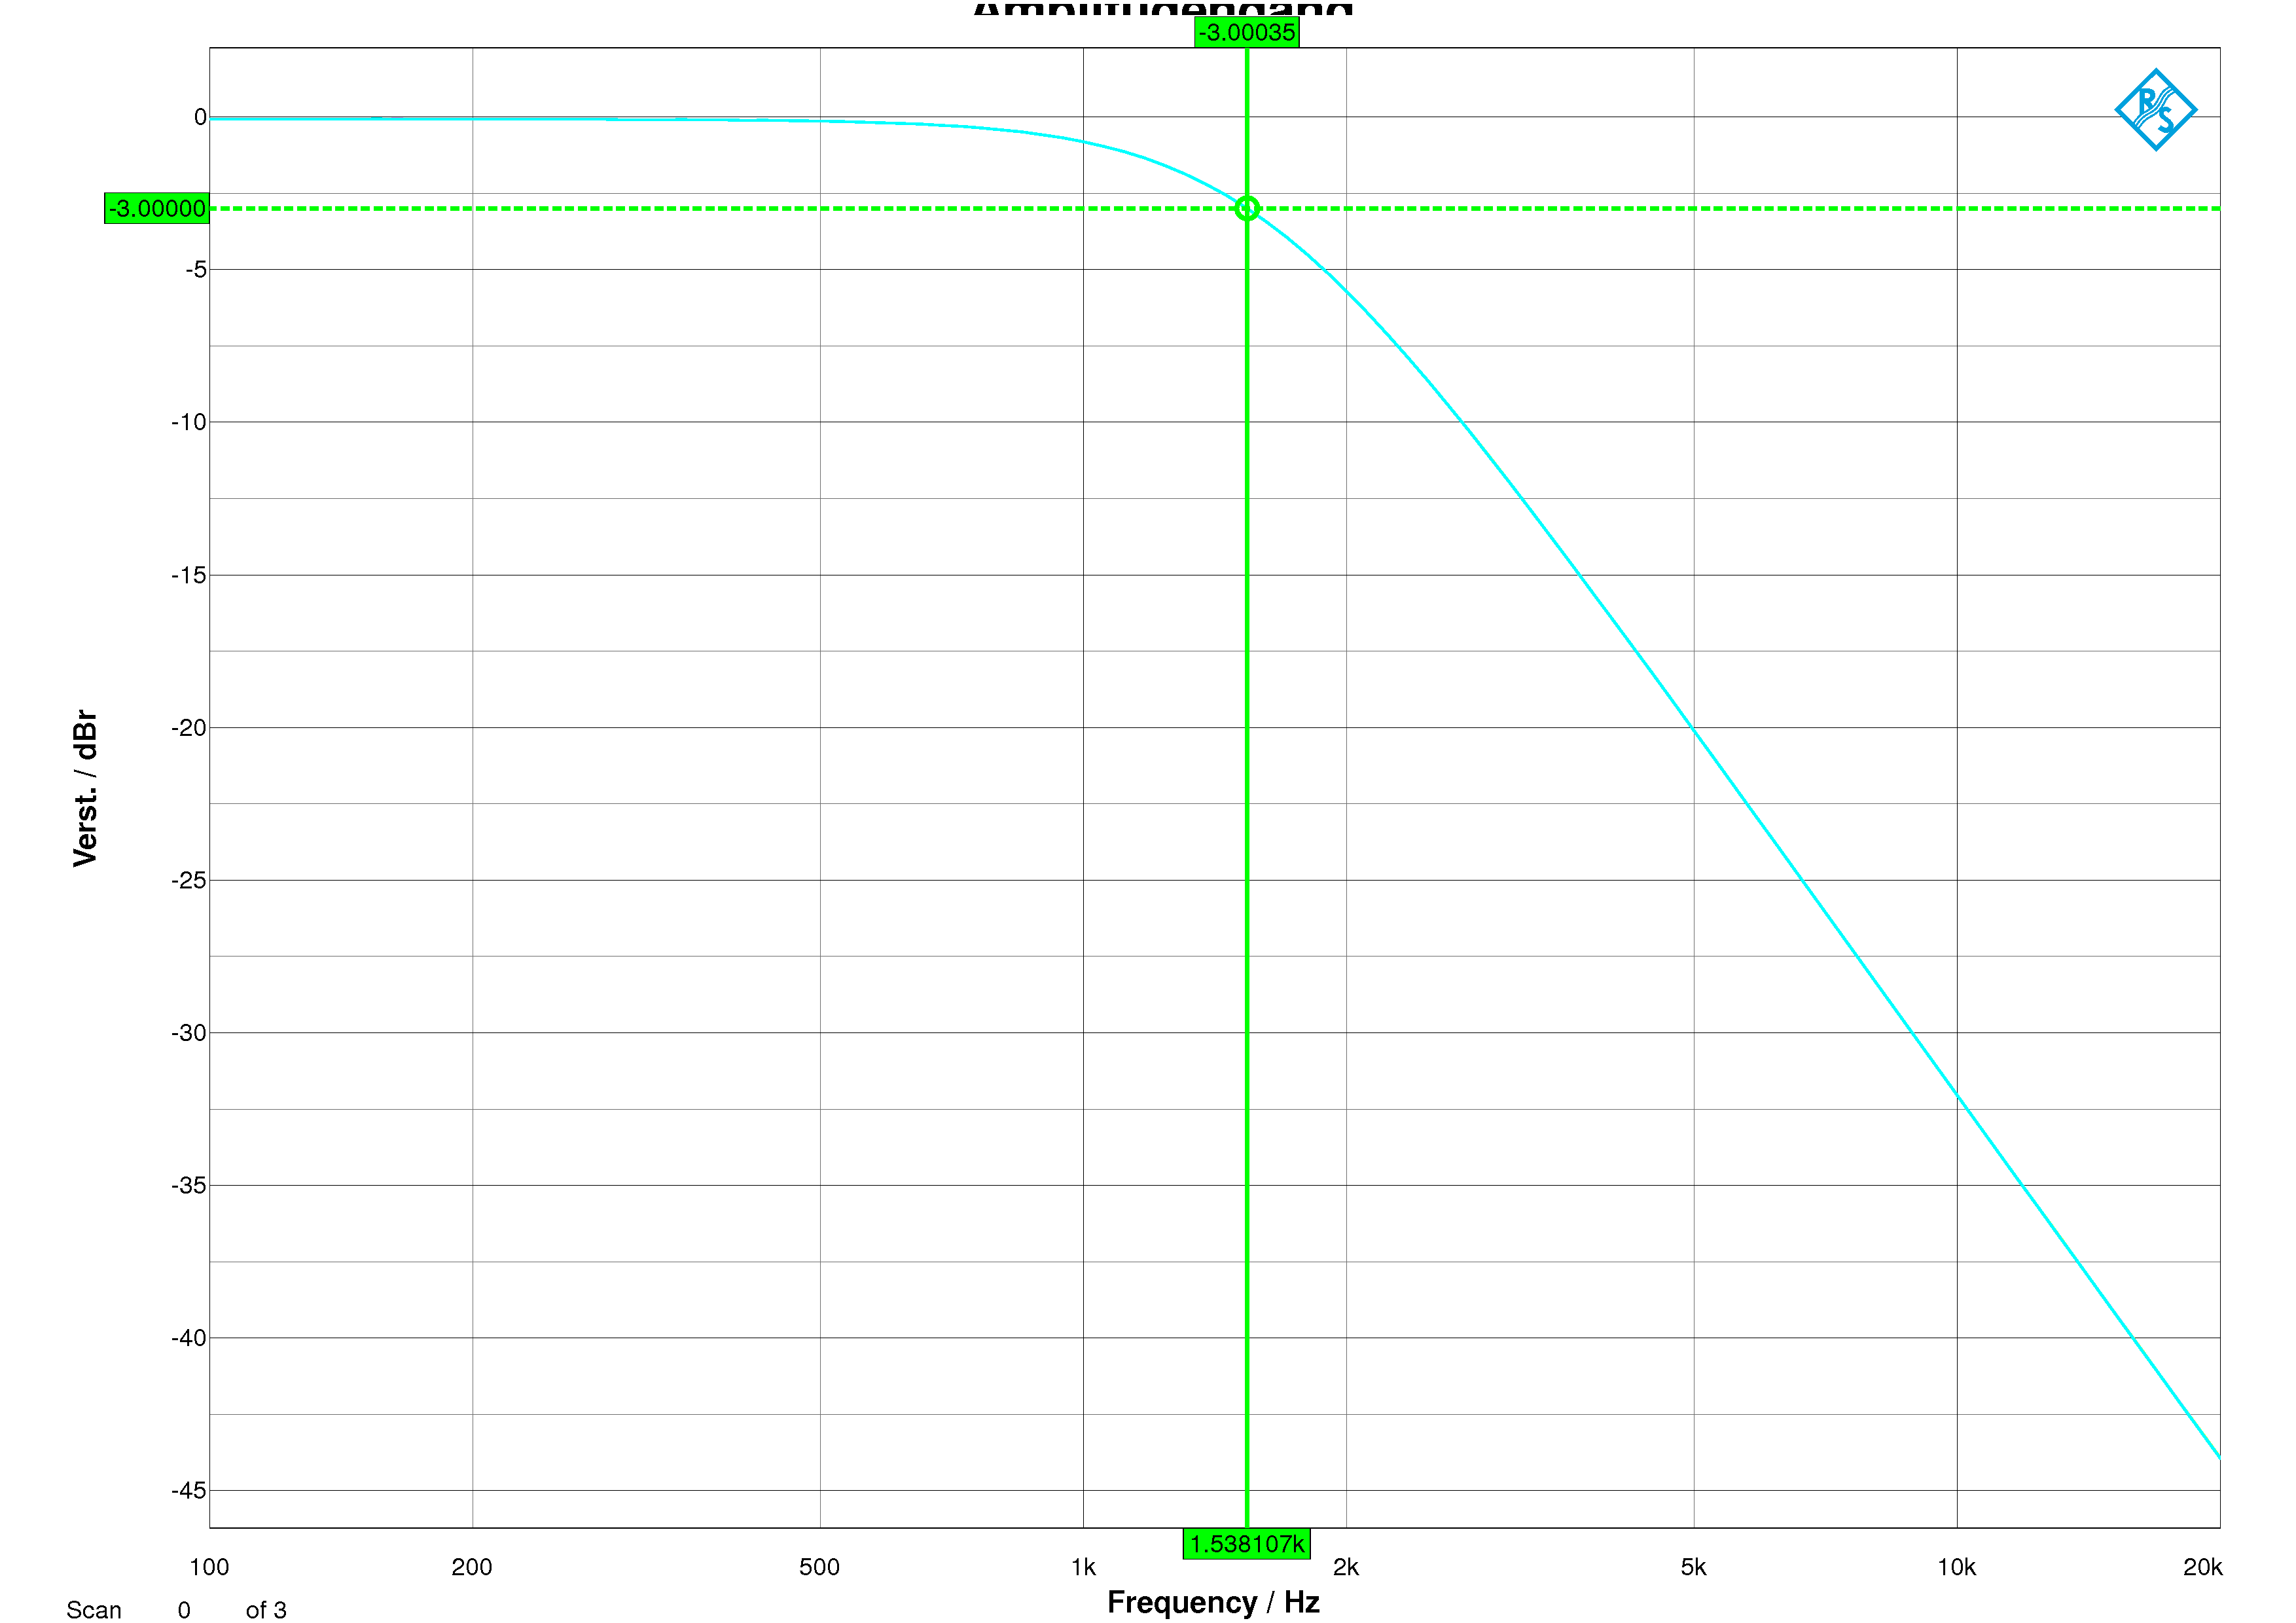
\includegraphics[width=0.64\linewidth]{Bilder/ImLabor/Amplitudengang_2_1_Butter_TP}
\caption{Amplitudengang Butterworth-Tiefpass mit Marker}
\label{fig:Amplitudengang_2_1_Butter_TP}
\end{figure}

\begin{figure}[h]
\centering
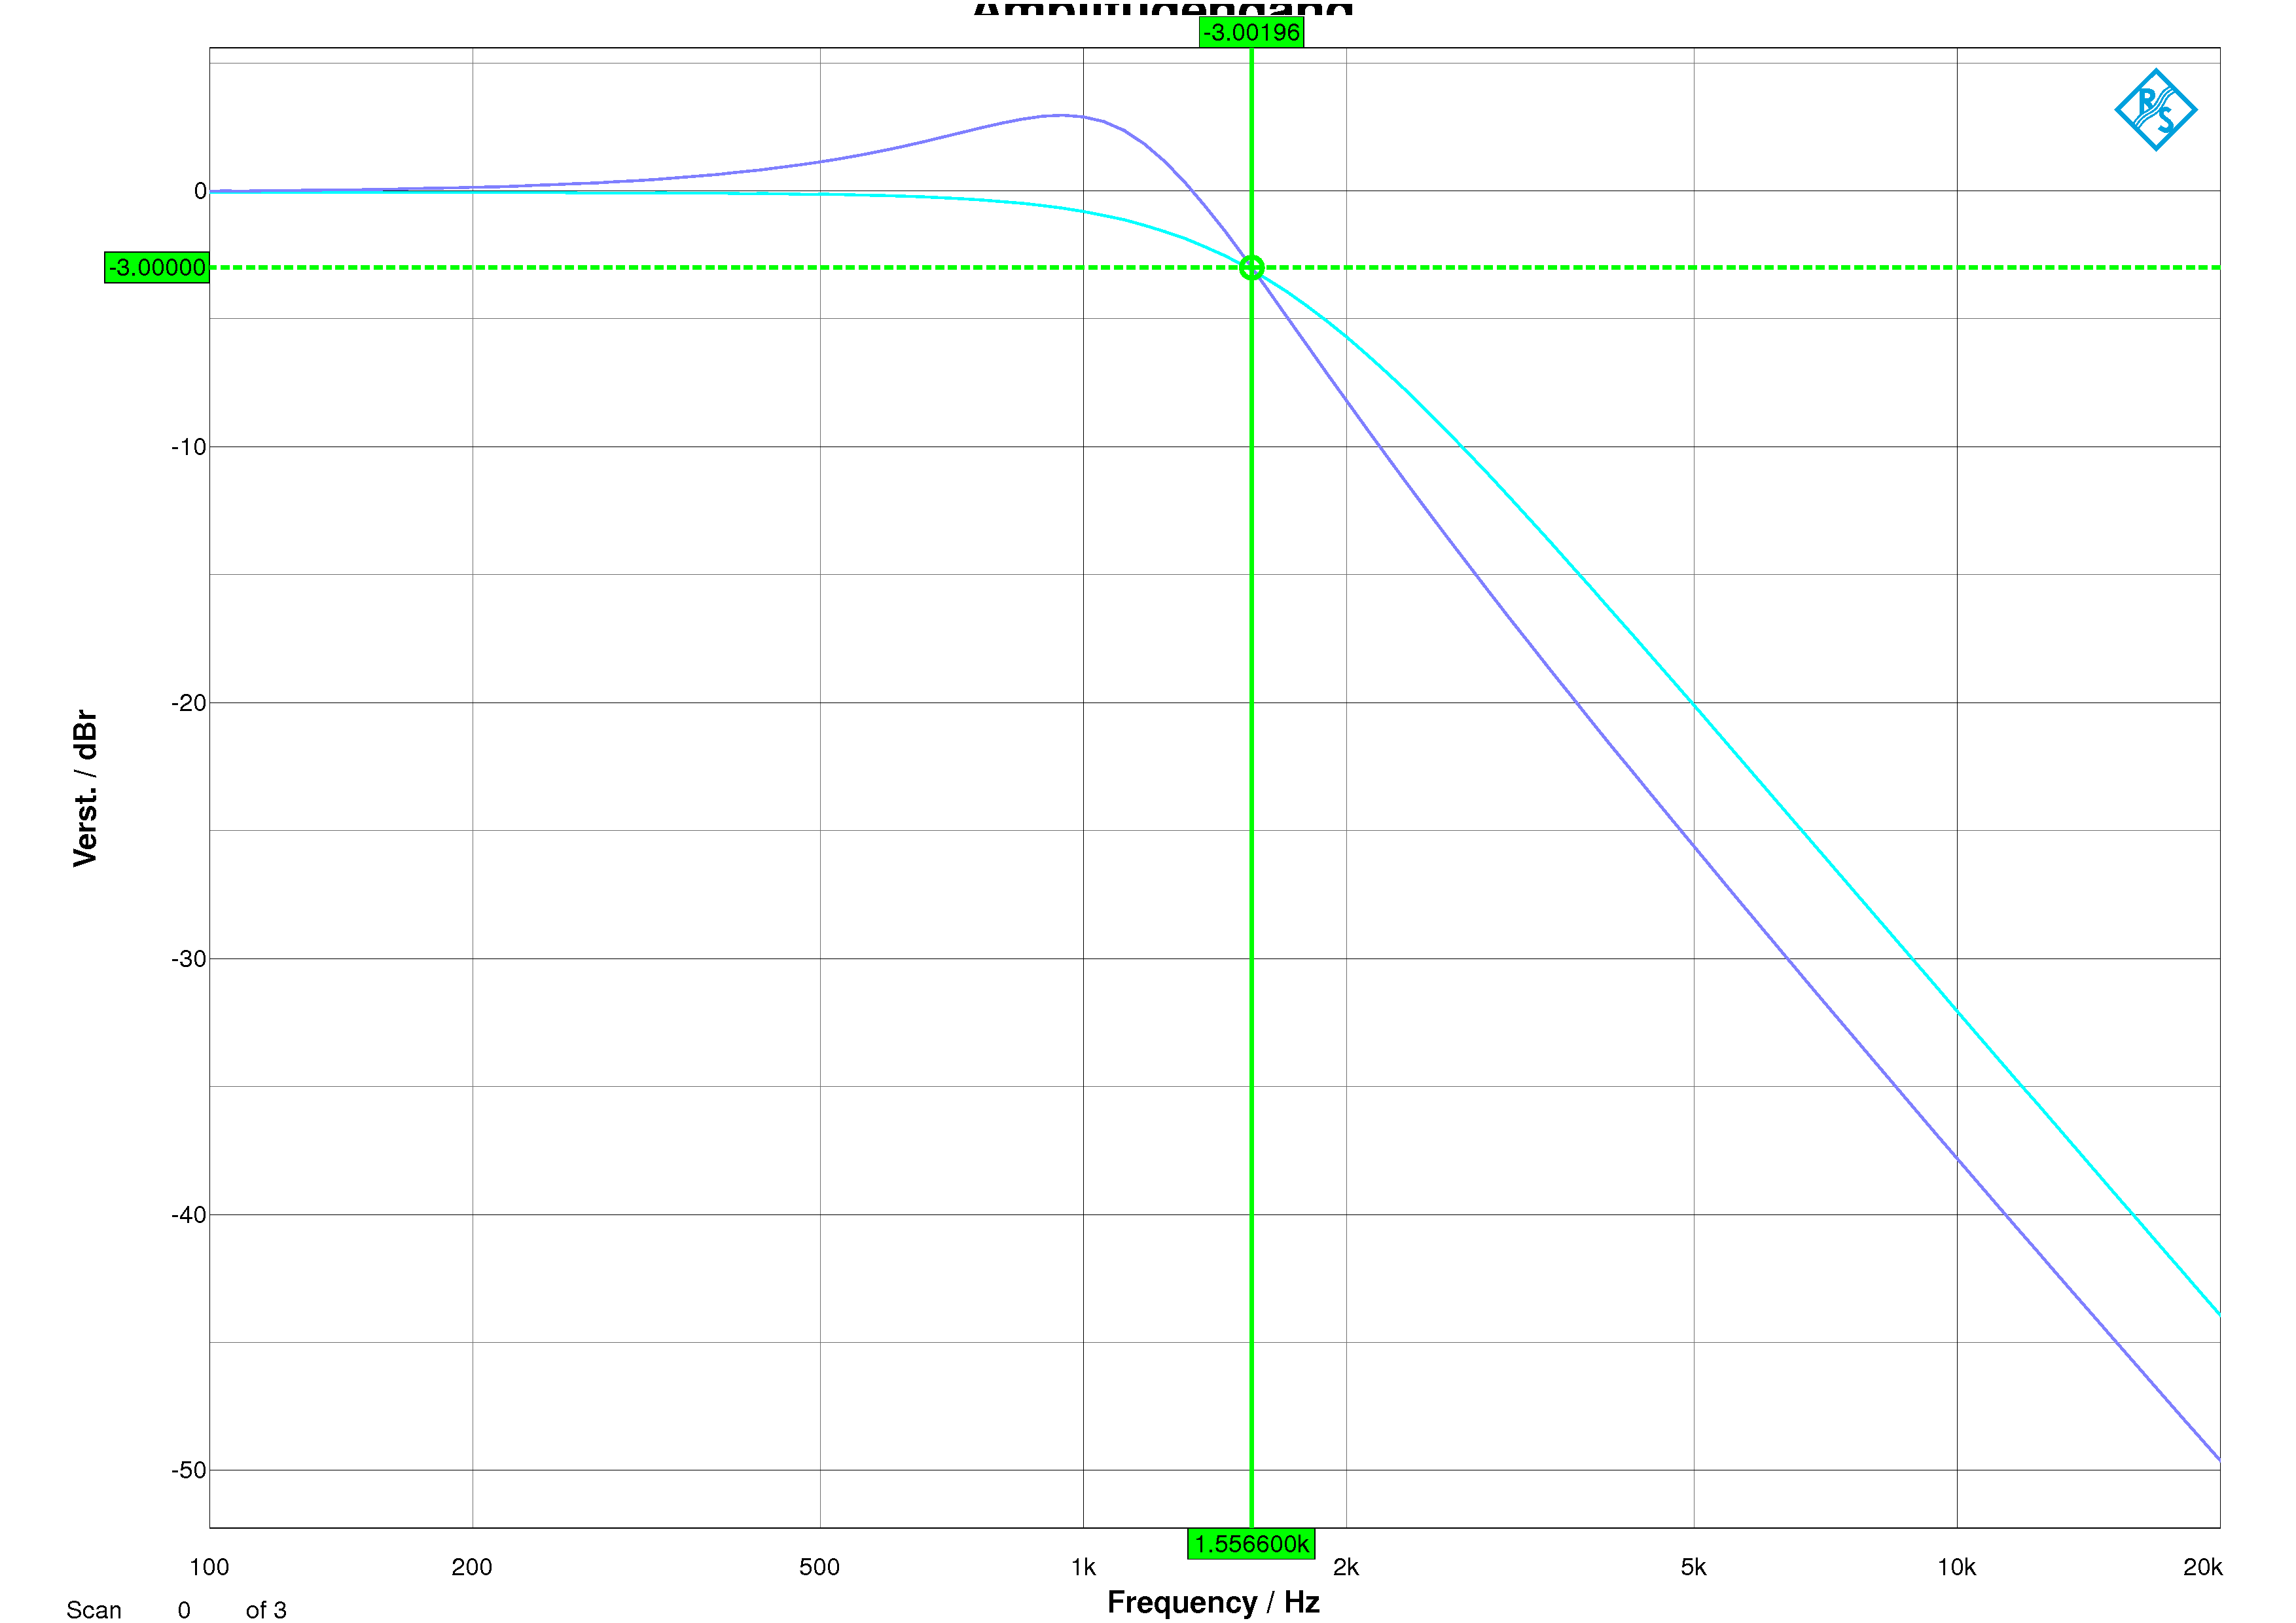
\includegraphics[width=0.65\linewidth]{Bilder/ImLabor/Amplitudengang_2_2_Tscheby_TP}
\caption{Amplitudengang Butterworth- und Tschebyscheff-Tiefpass mit Marker bei Tschebyscheff}
\label{fig:Amplitudengang_2_2_Tscheby_TP}
\end{figure}

\begin{figure}[h]
\centering
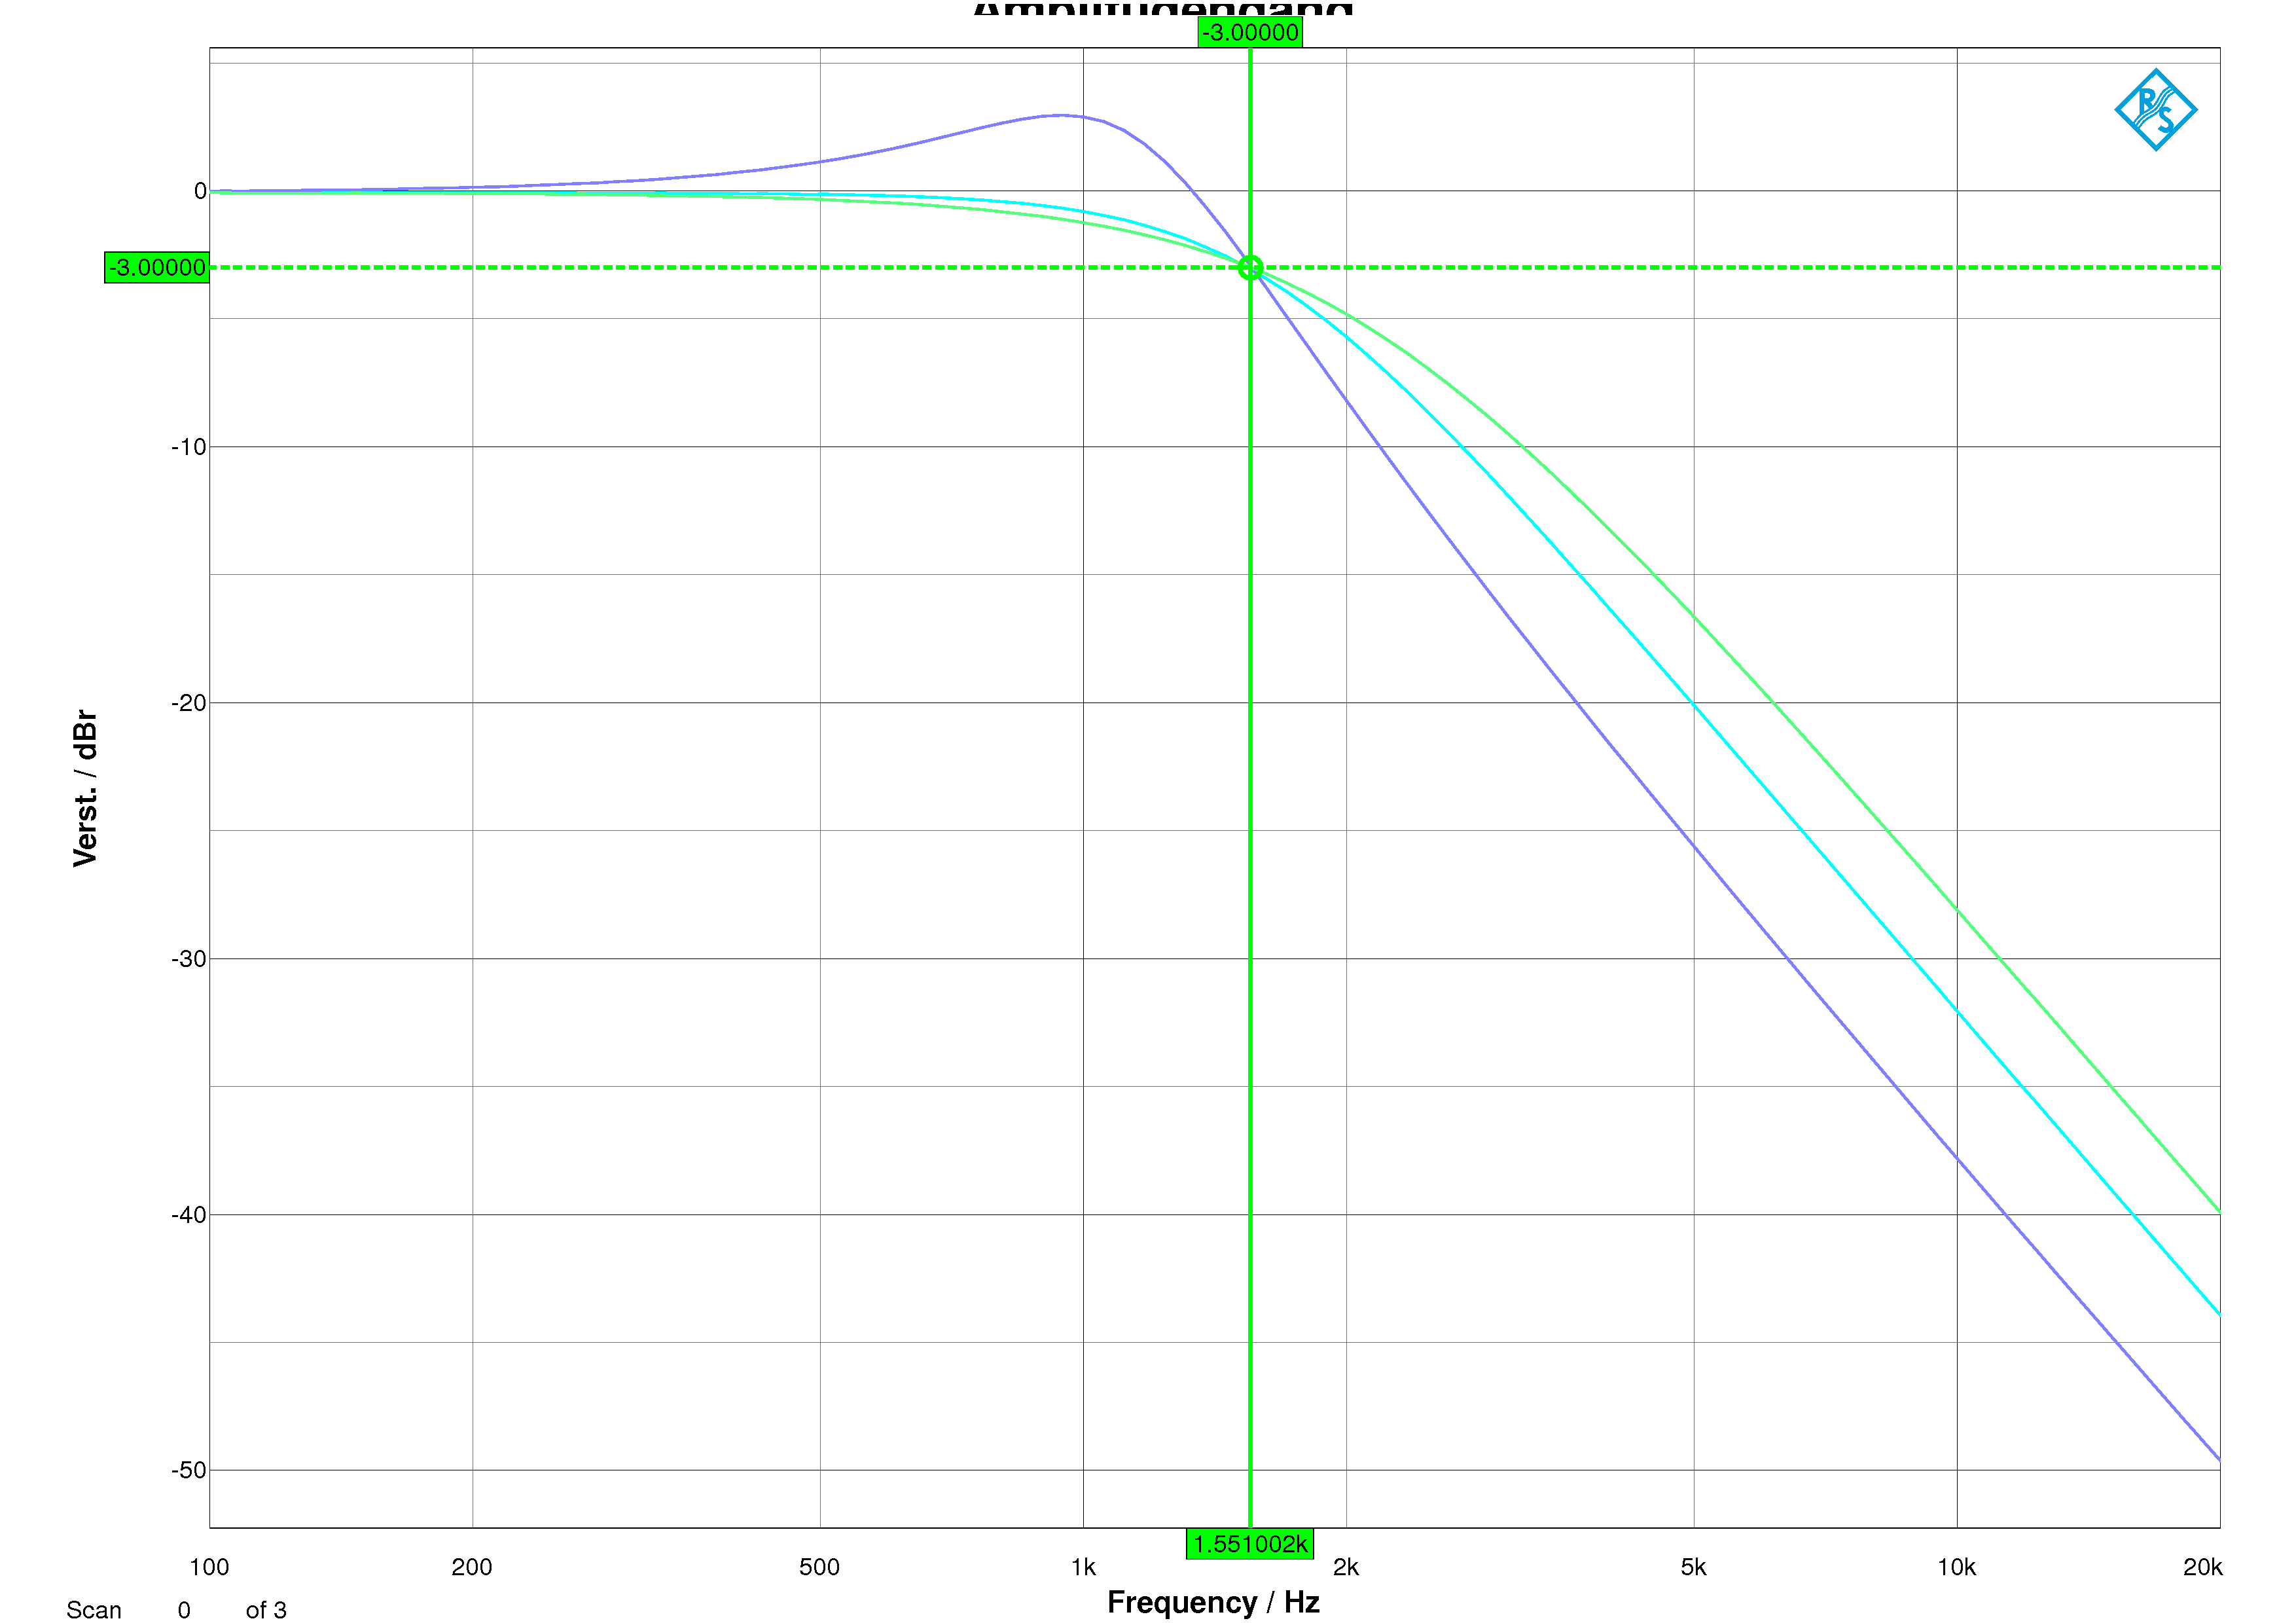
\includegraphics[width=0.65\linewidth]{Bilder/ImLabor/Amplitudengang_2_3_Bessel_TP_Alle}
\caption{Amplitudengang Butterworth-, Tschebyscheff- und Bessel-Tiefpass mit Marker bei Bessel}
\label{fig:Amplitudengang_2_3_Bessel_TP_Alle}
\end{figure}

\begin{figure}[h]
\centering
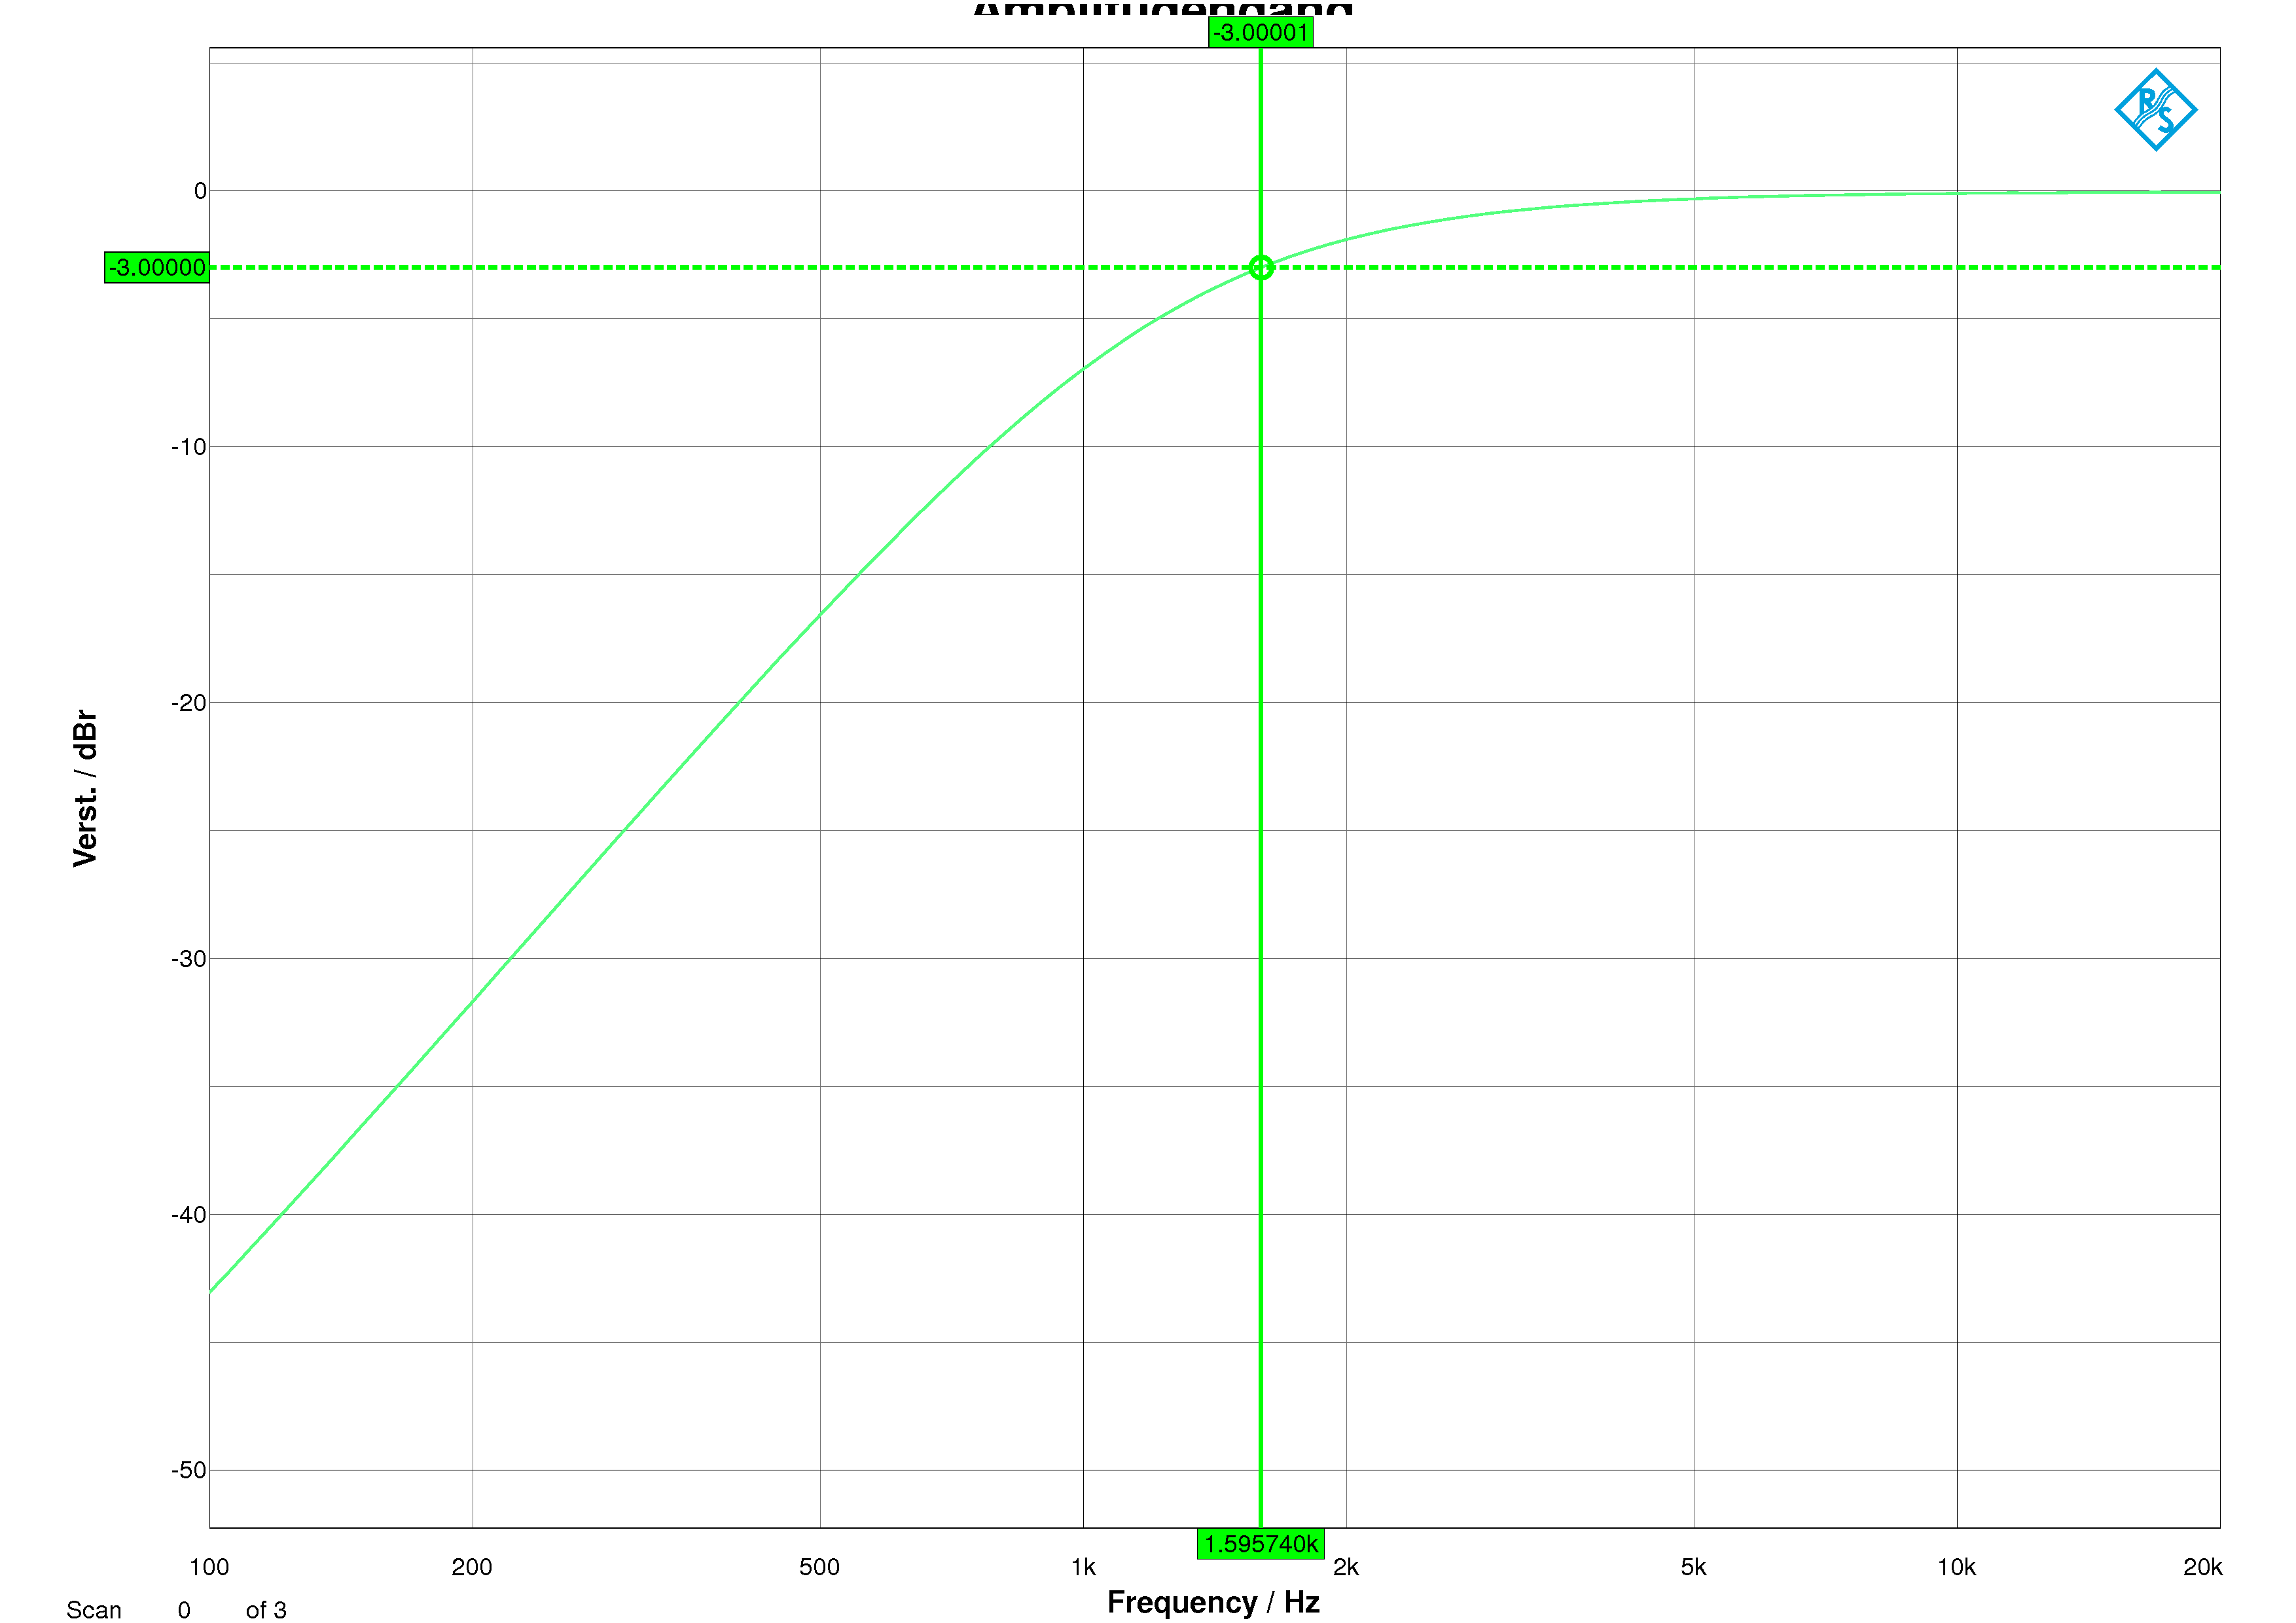
\includegraphics[width=0.65\linewidth]{Bilder/ImLabor/Amplitudengang_1_1_Butter_HP}
\caption{Amplitudengang Butterworth-Hochpass mit Marker}
\label{fig:Amplitudengang_1_1_Butter_HP}
\end{figure}

\begin{figure}[h]
\centering
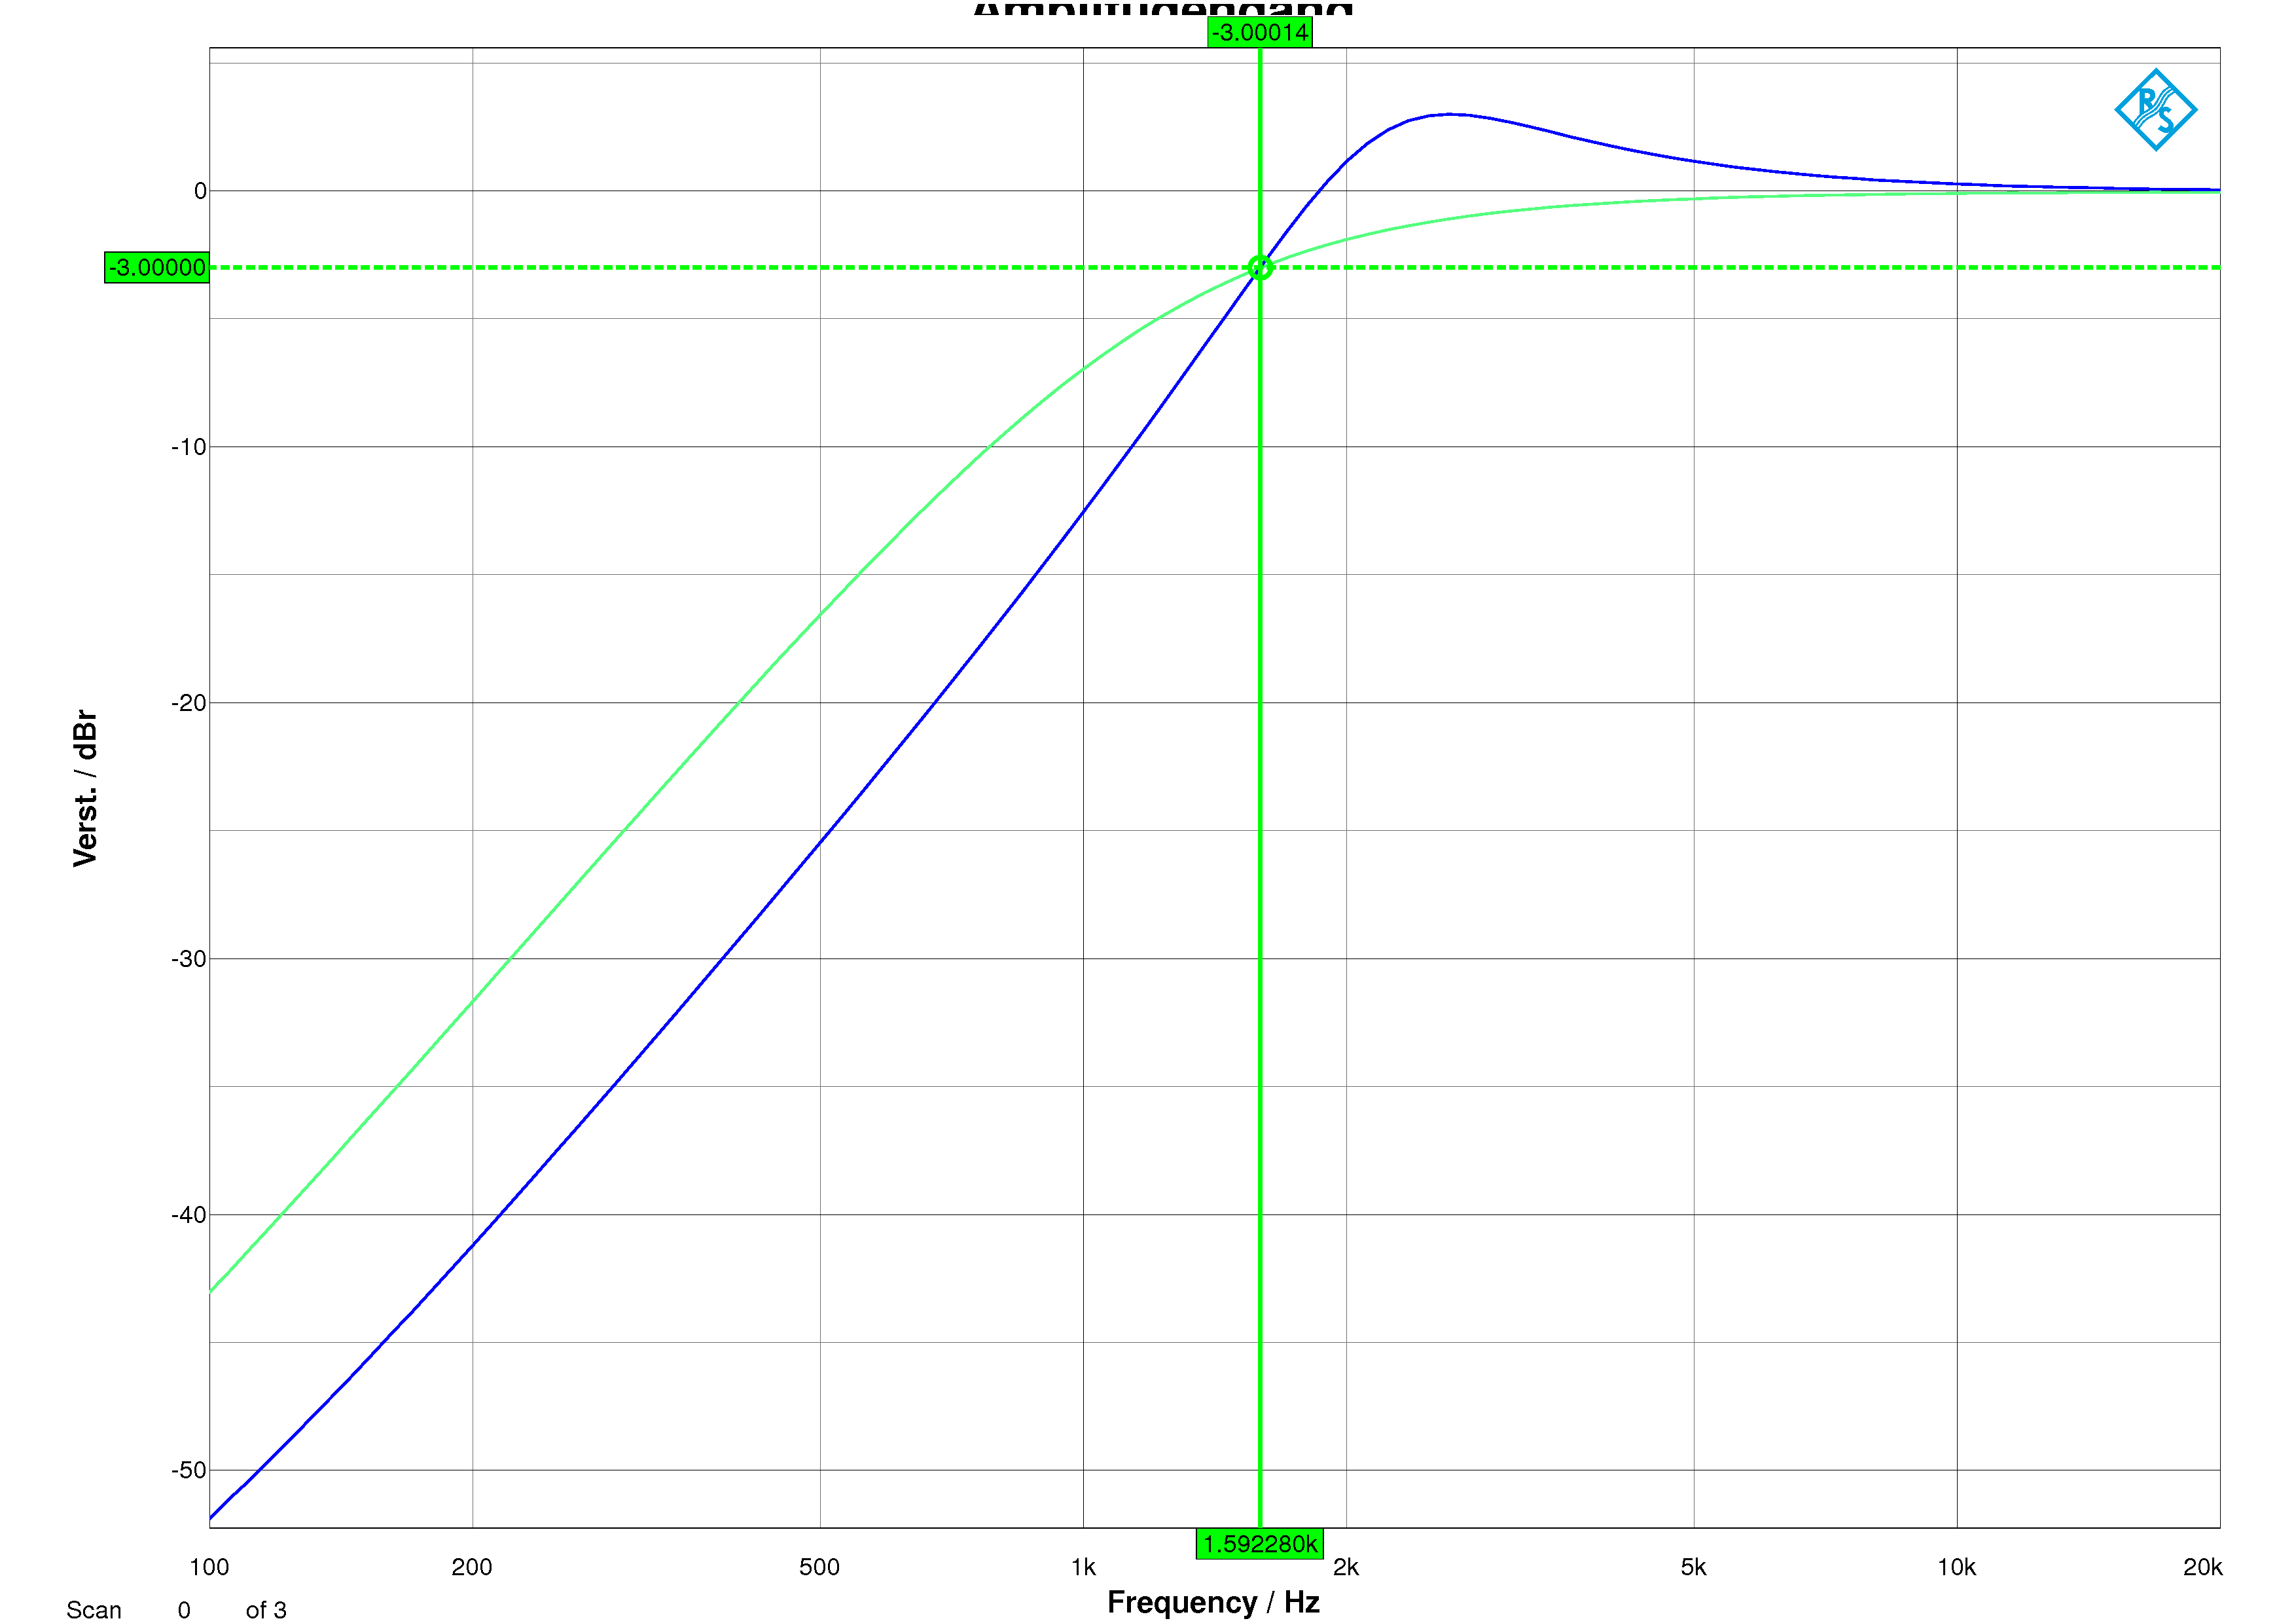
\includegraphics[width=0.65\linewidth]{Bilder/ImLabor/Amplitudengang_1_2_Tscheby_HP}
\caption{Amplitudengang Butterworth- und Tschebyscheff-Hochpass mit Marker bei Tschebyscheff}
\label{fig:Amplitudengang_1_2_Tscheby_HP}
\end{figure}

\begin{figure}[h]
\centering
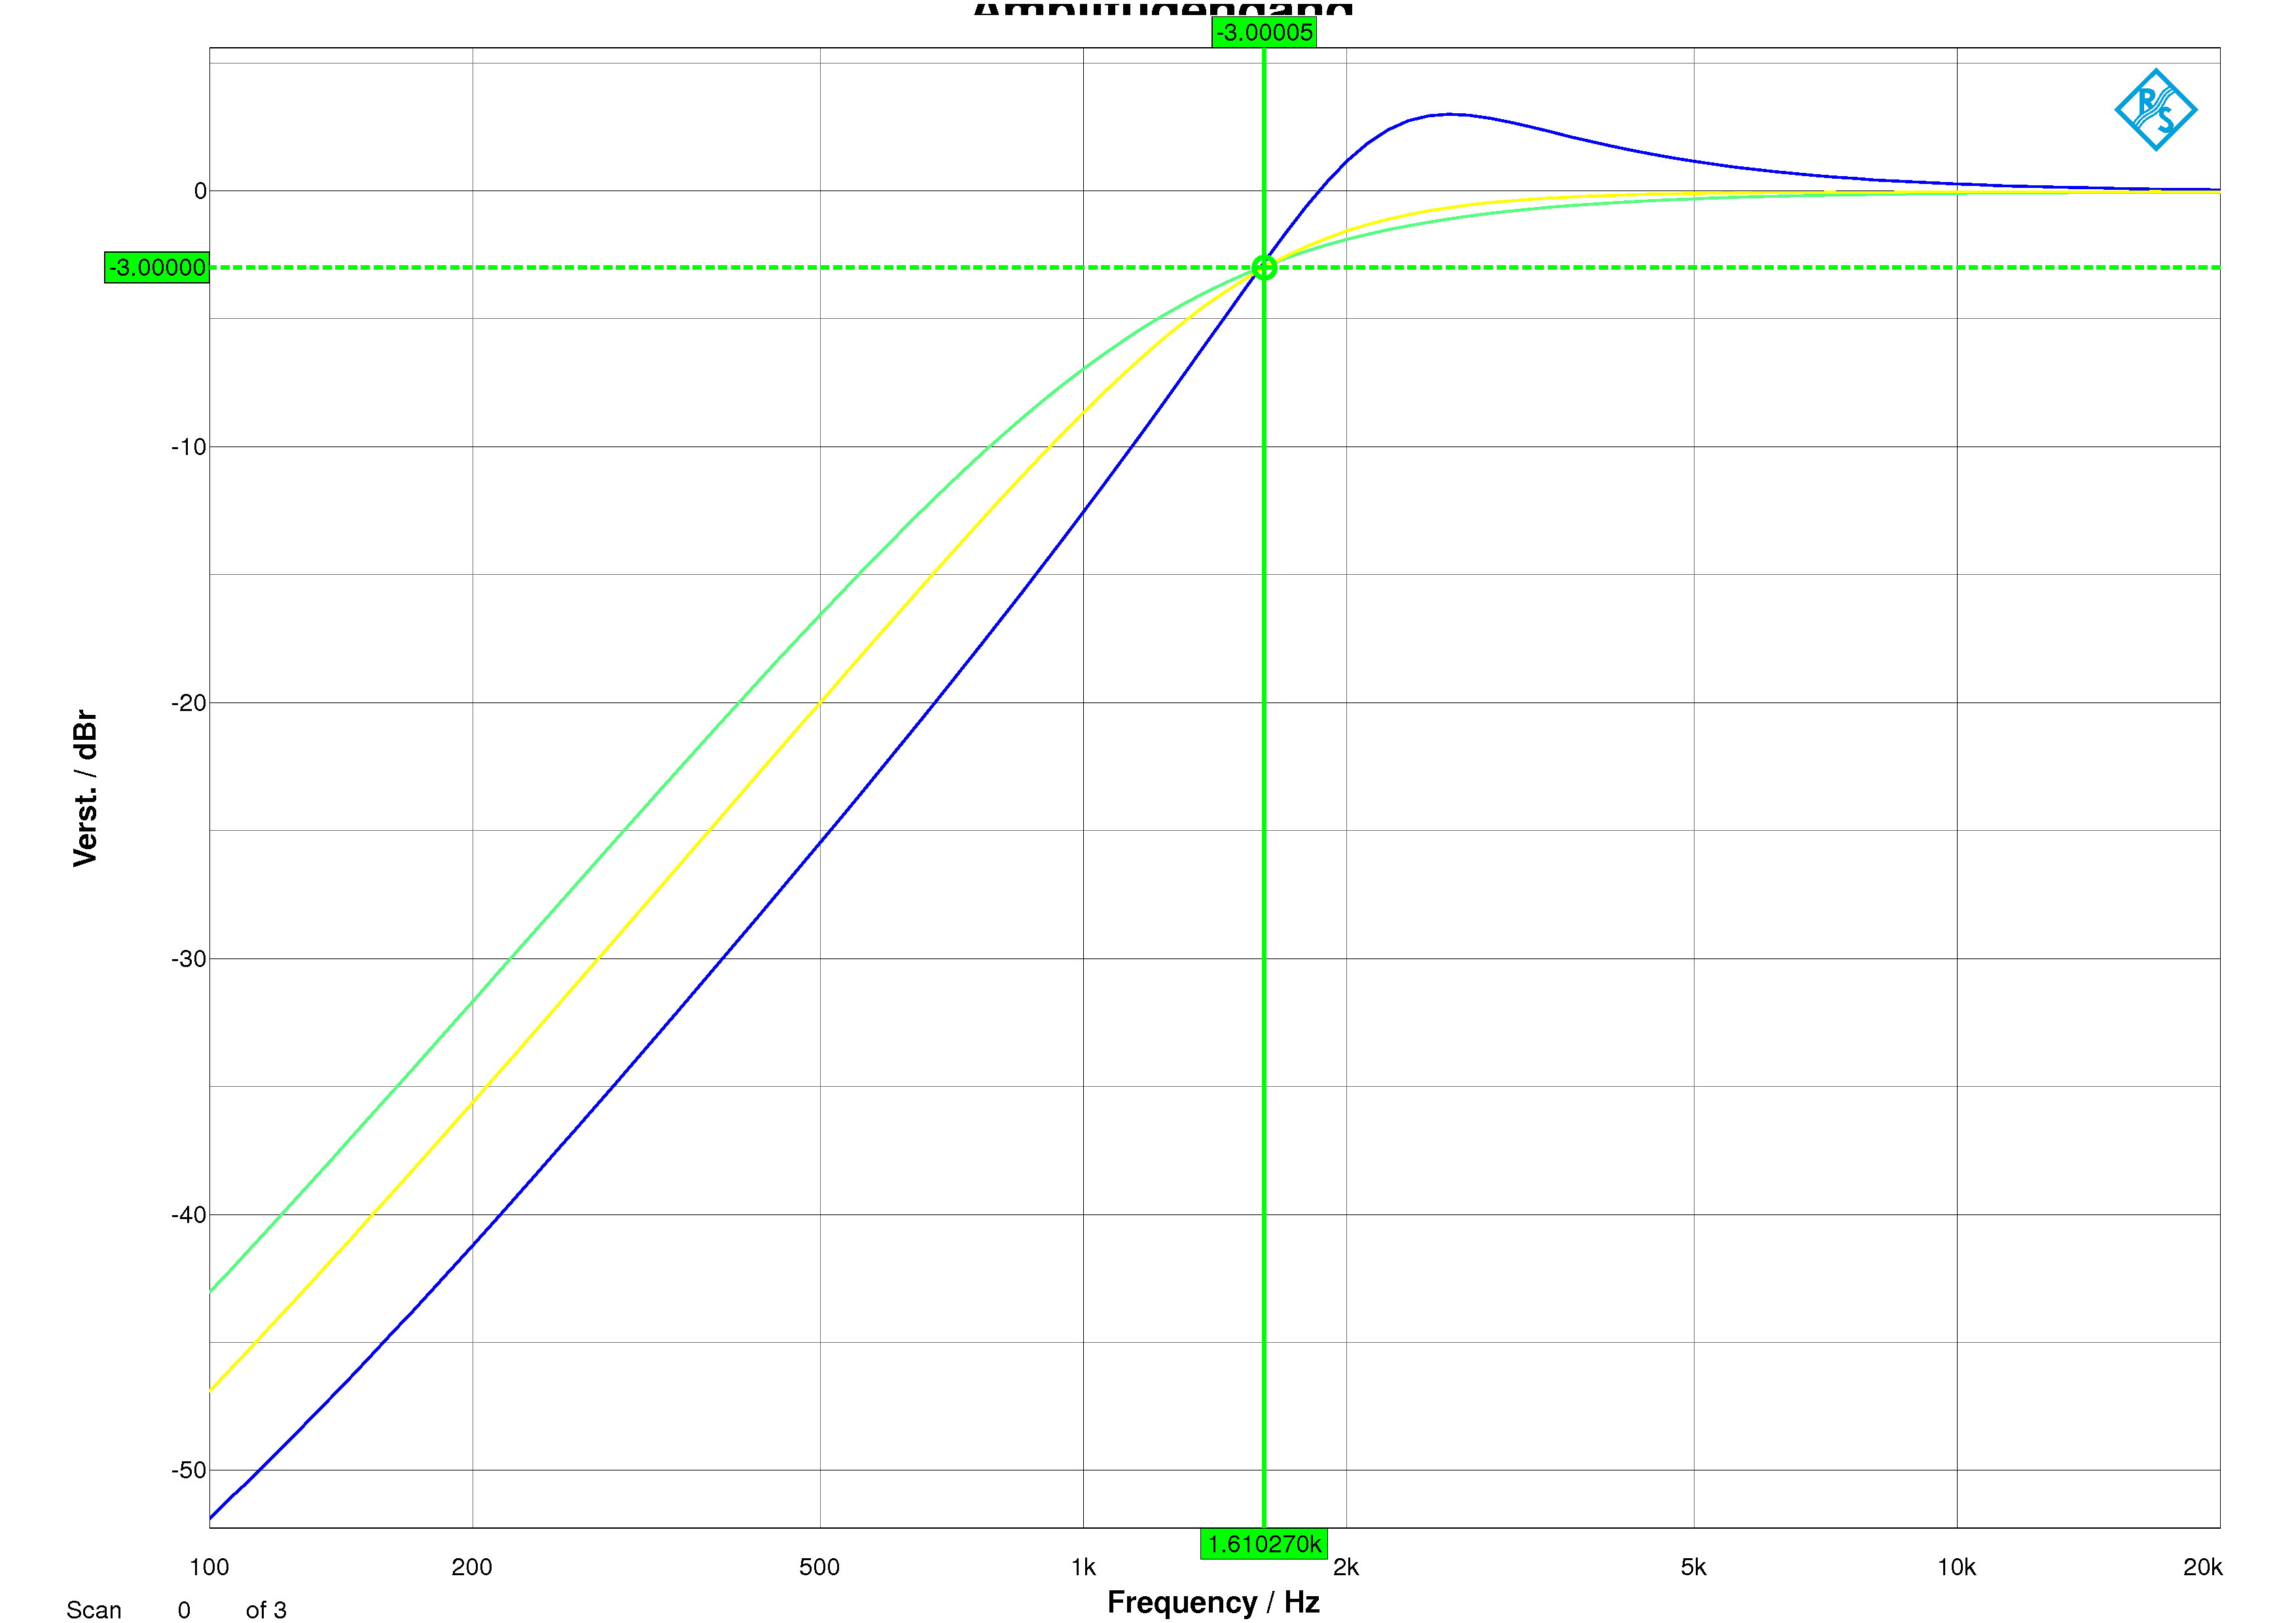
\includegraphics[width=0.65\linewidth]{Bilder/ImLabor/Amplitudengang_1_3_Bessel_HP_Alle}
\caption{Amplitudengang Butterworth-, Tschebyscheff- und Bessel-Hochpass mit Marker bei Bessel}
\label{fig:Amplitudengang_1_3_Bessel_HP_Alle}
\end{figure}

\begin{figure}[h]
\centering
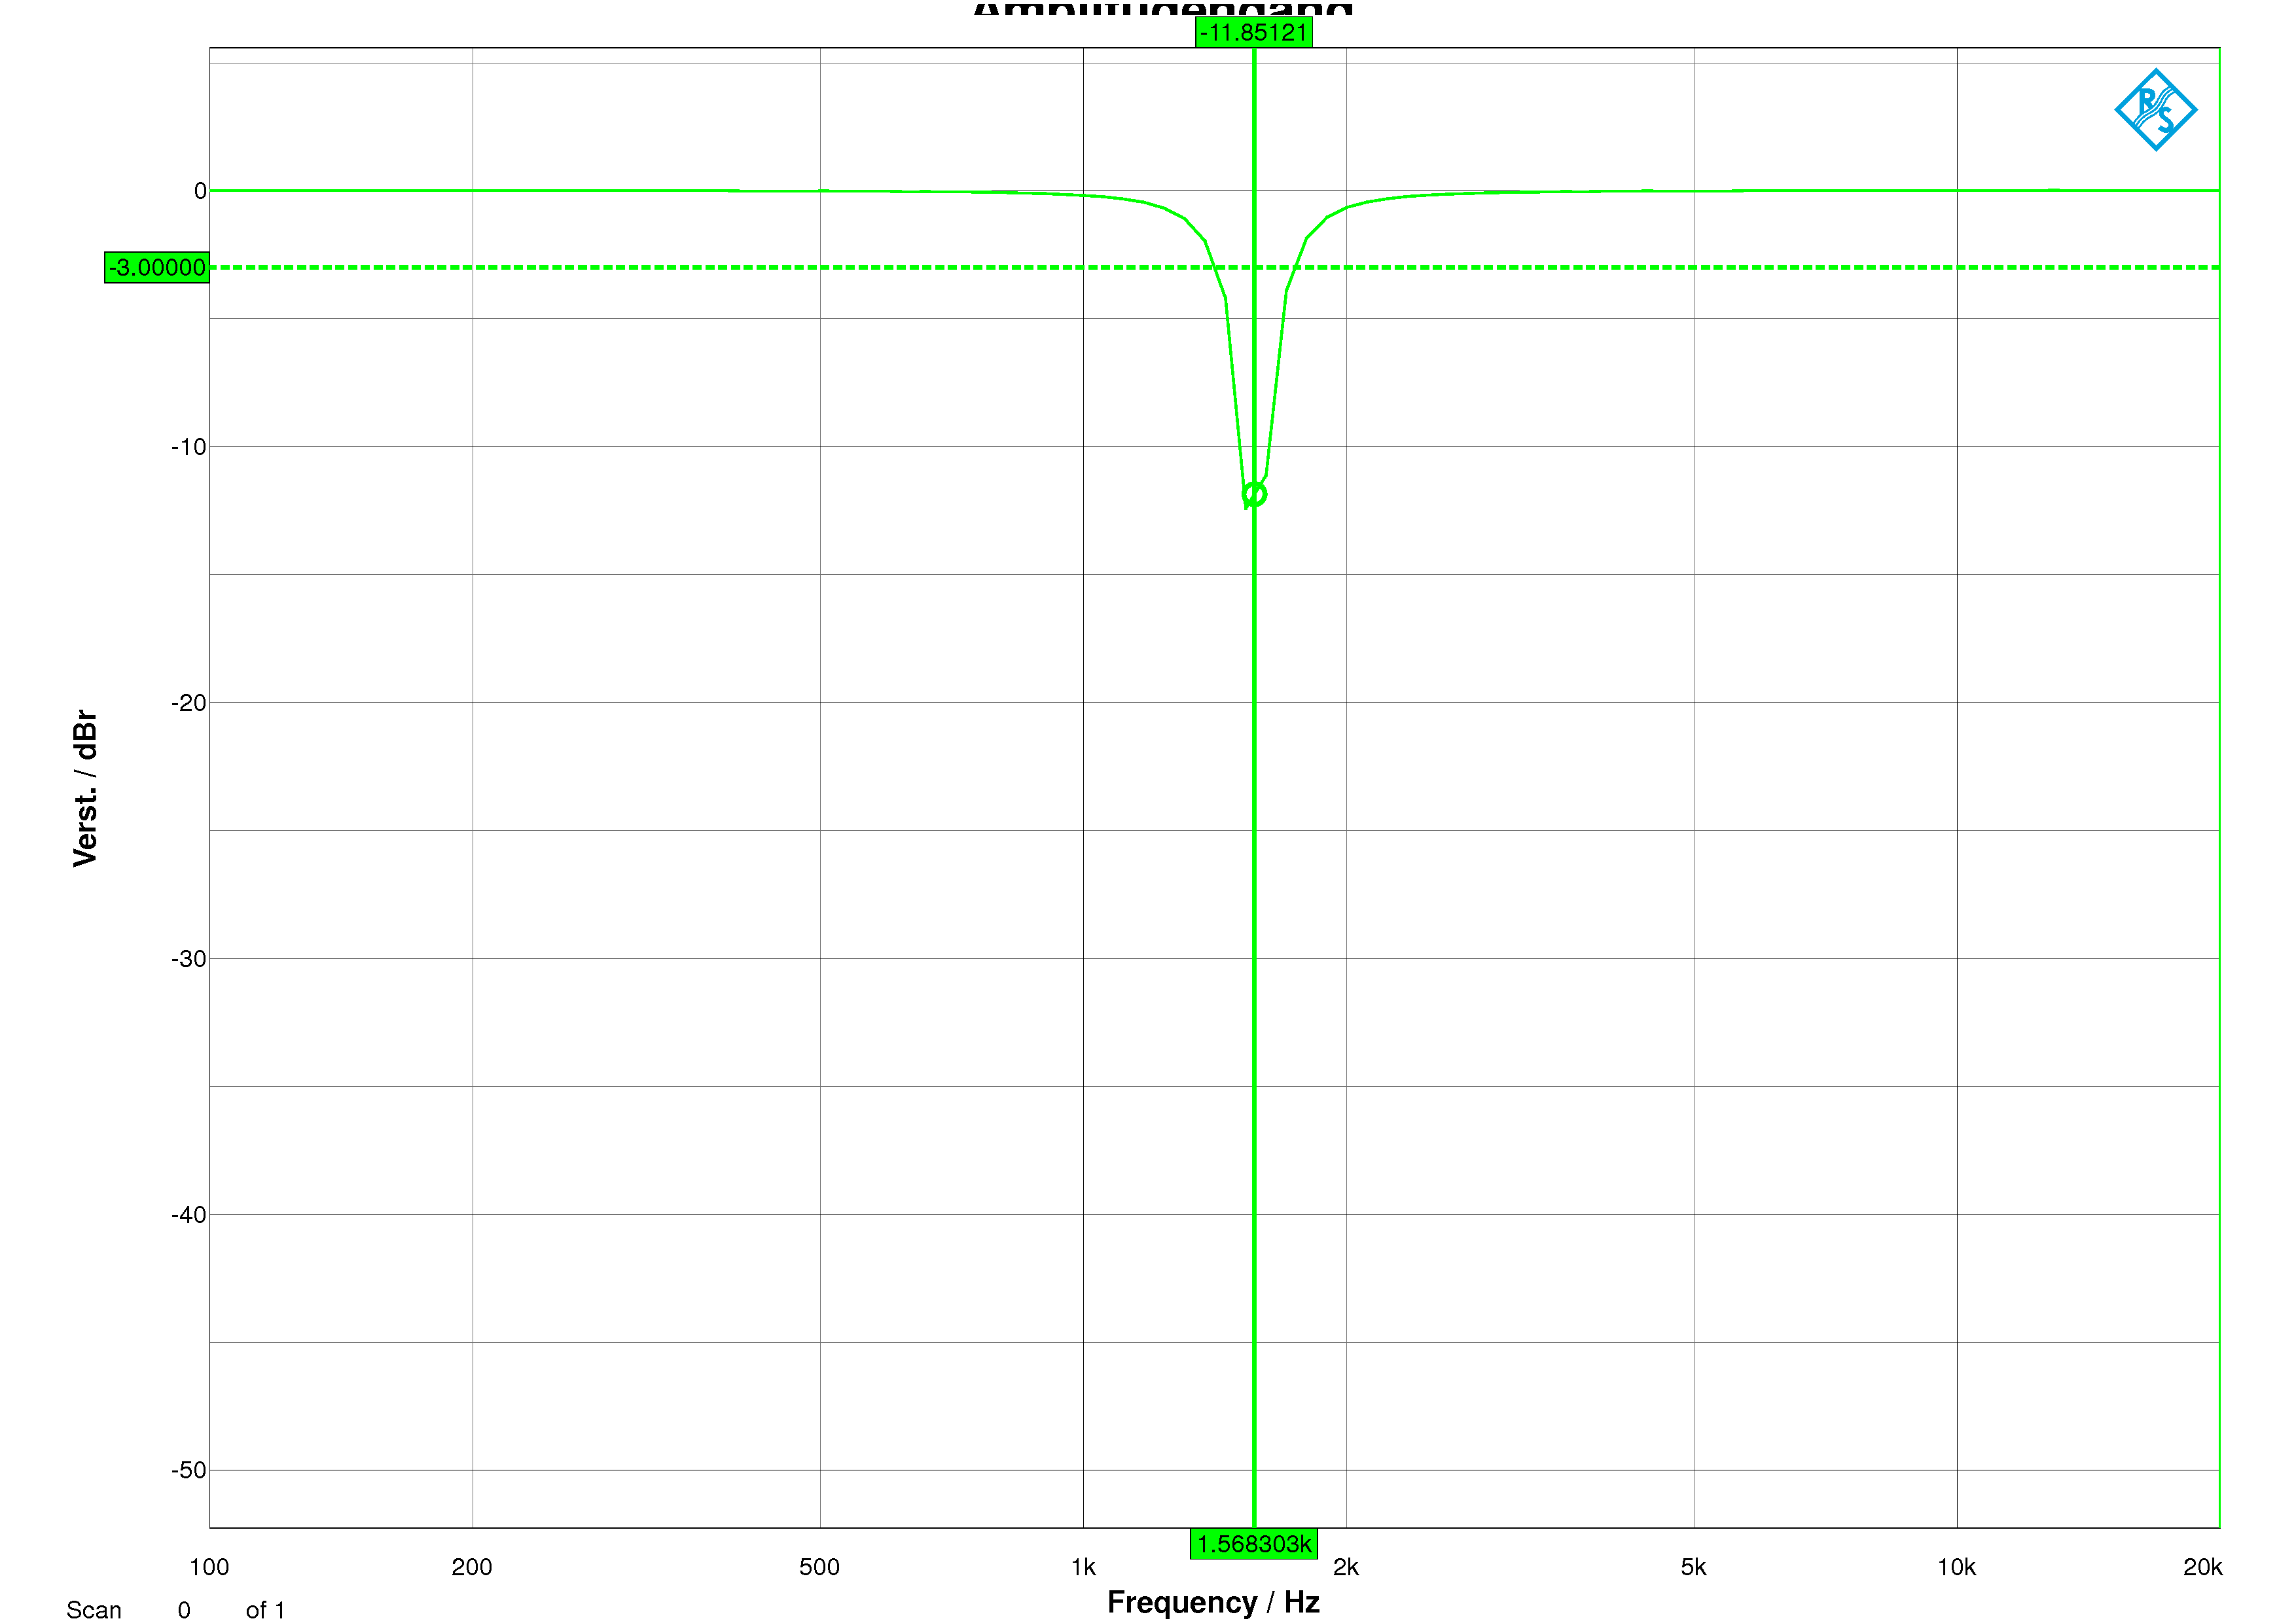
\includegraphics[width=0.65\linewidth]{Bilder/ImLabor/Amplitudengang_3_2_BS}
\caption{Amplitudengang Bandsperre mit Marker}
\label{fig:Amplitudengang_3_2_BS}
\end{figure}

\begin{figure}[h]
\centering
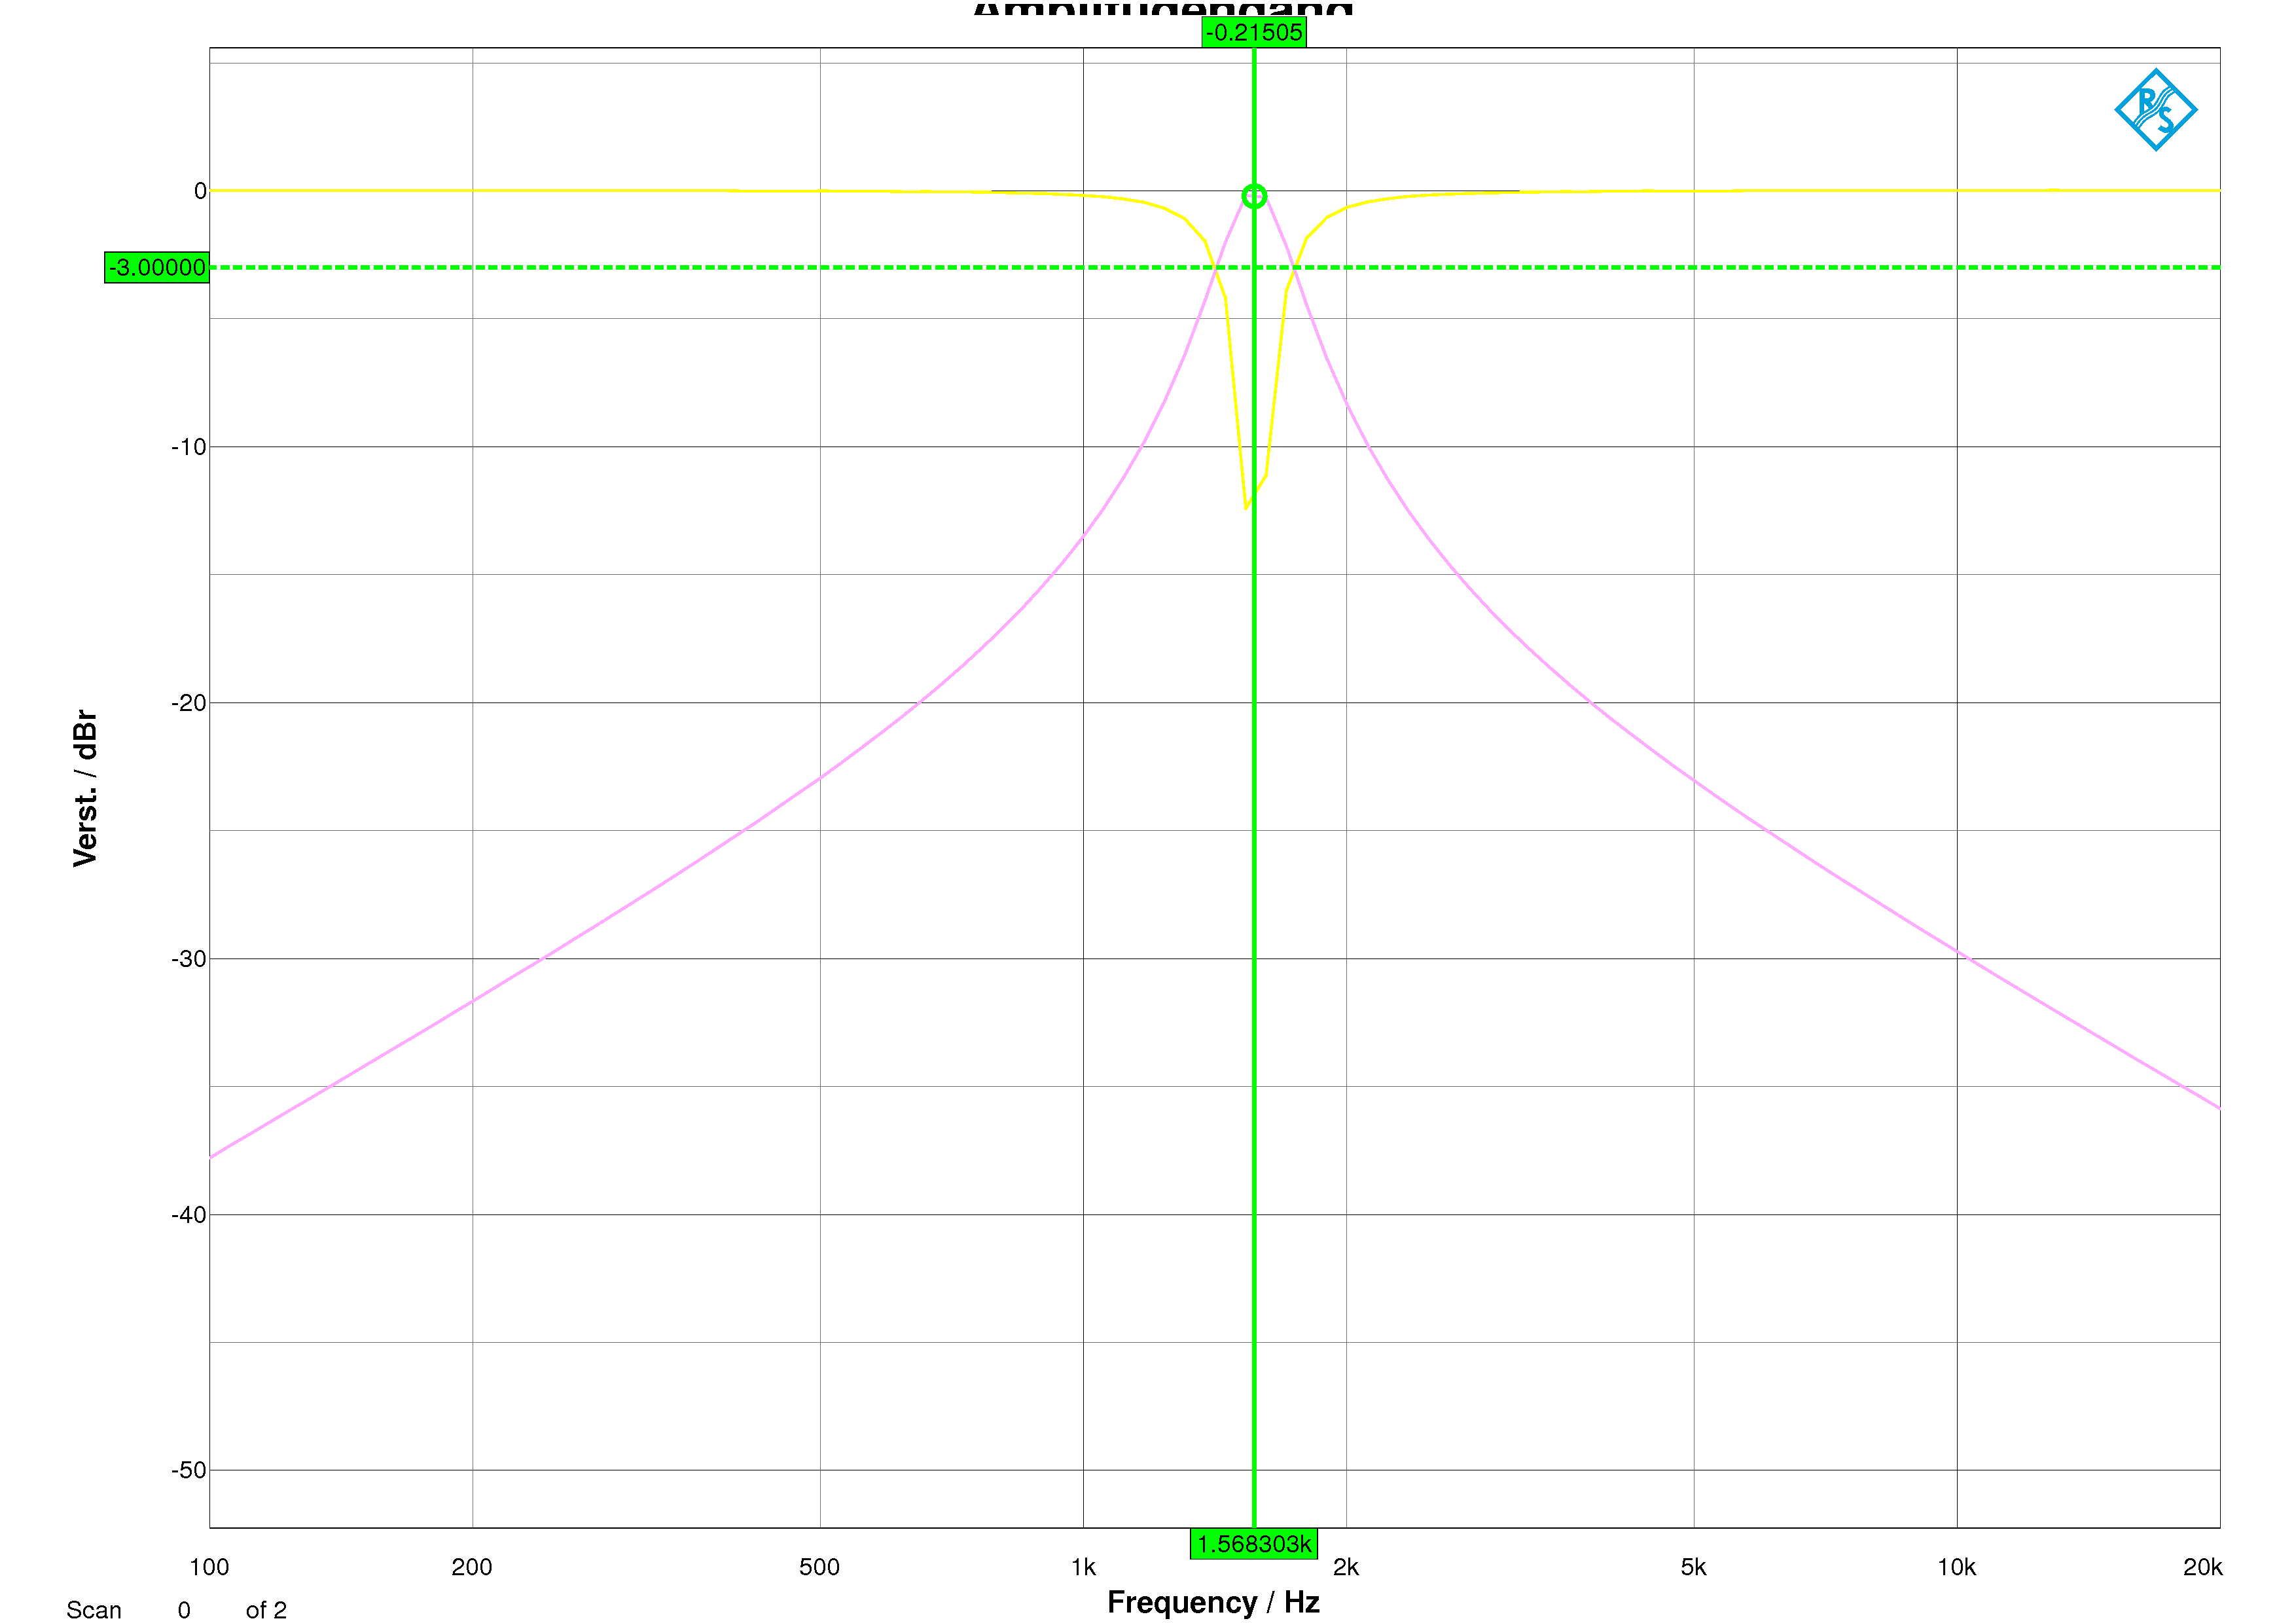
\includegraphics[width=0.65\linewidth]{Bilder/ImLabor/Amplitudengang_3_3_BP_BS}
\caption{Amplitudengang Bandsperre und Bandpass mit Maker beim Bandpass}
\label{fig:Amplitudengang_3_3_BP_BS}
\end{figure}

\begin{figure}[h]
\centering
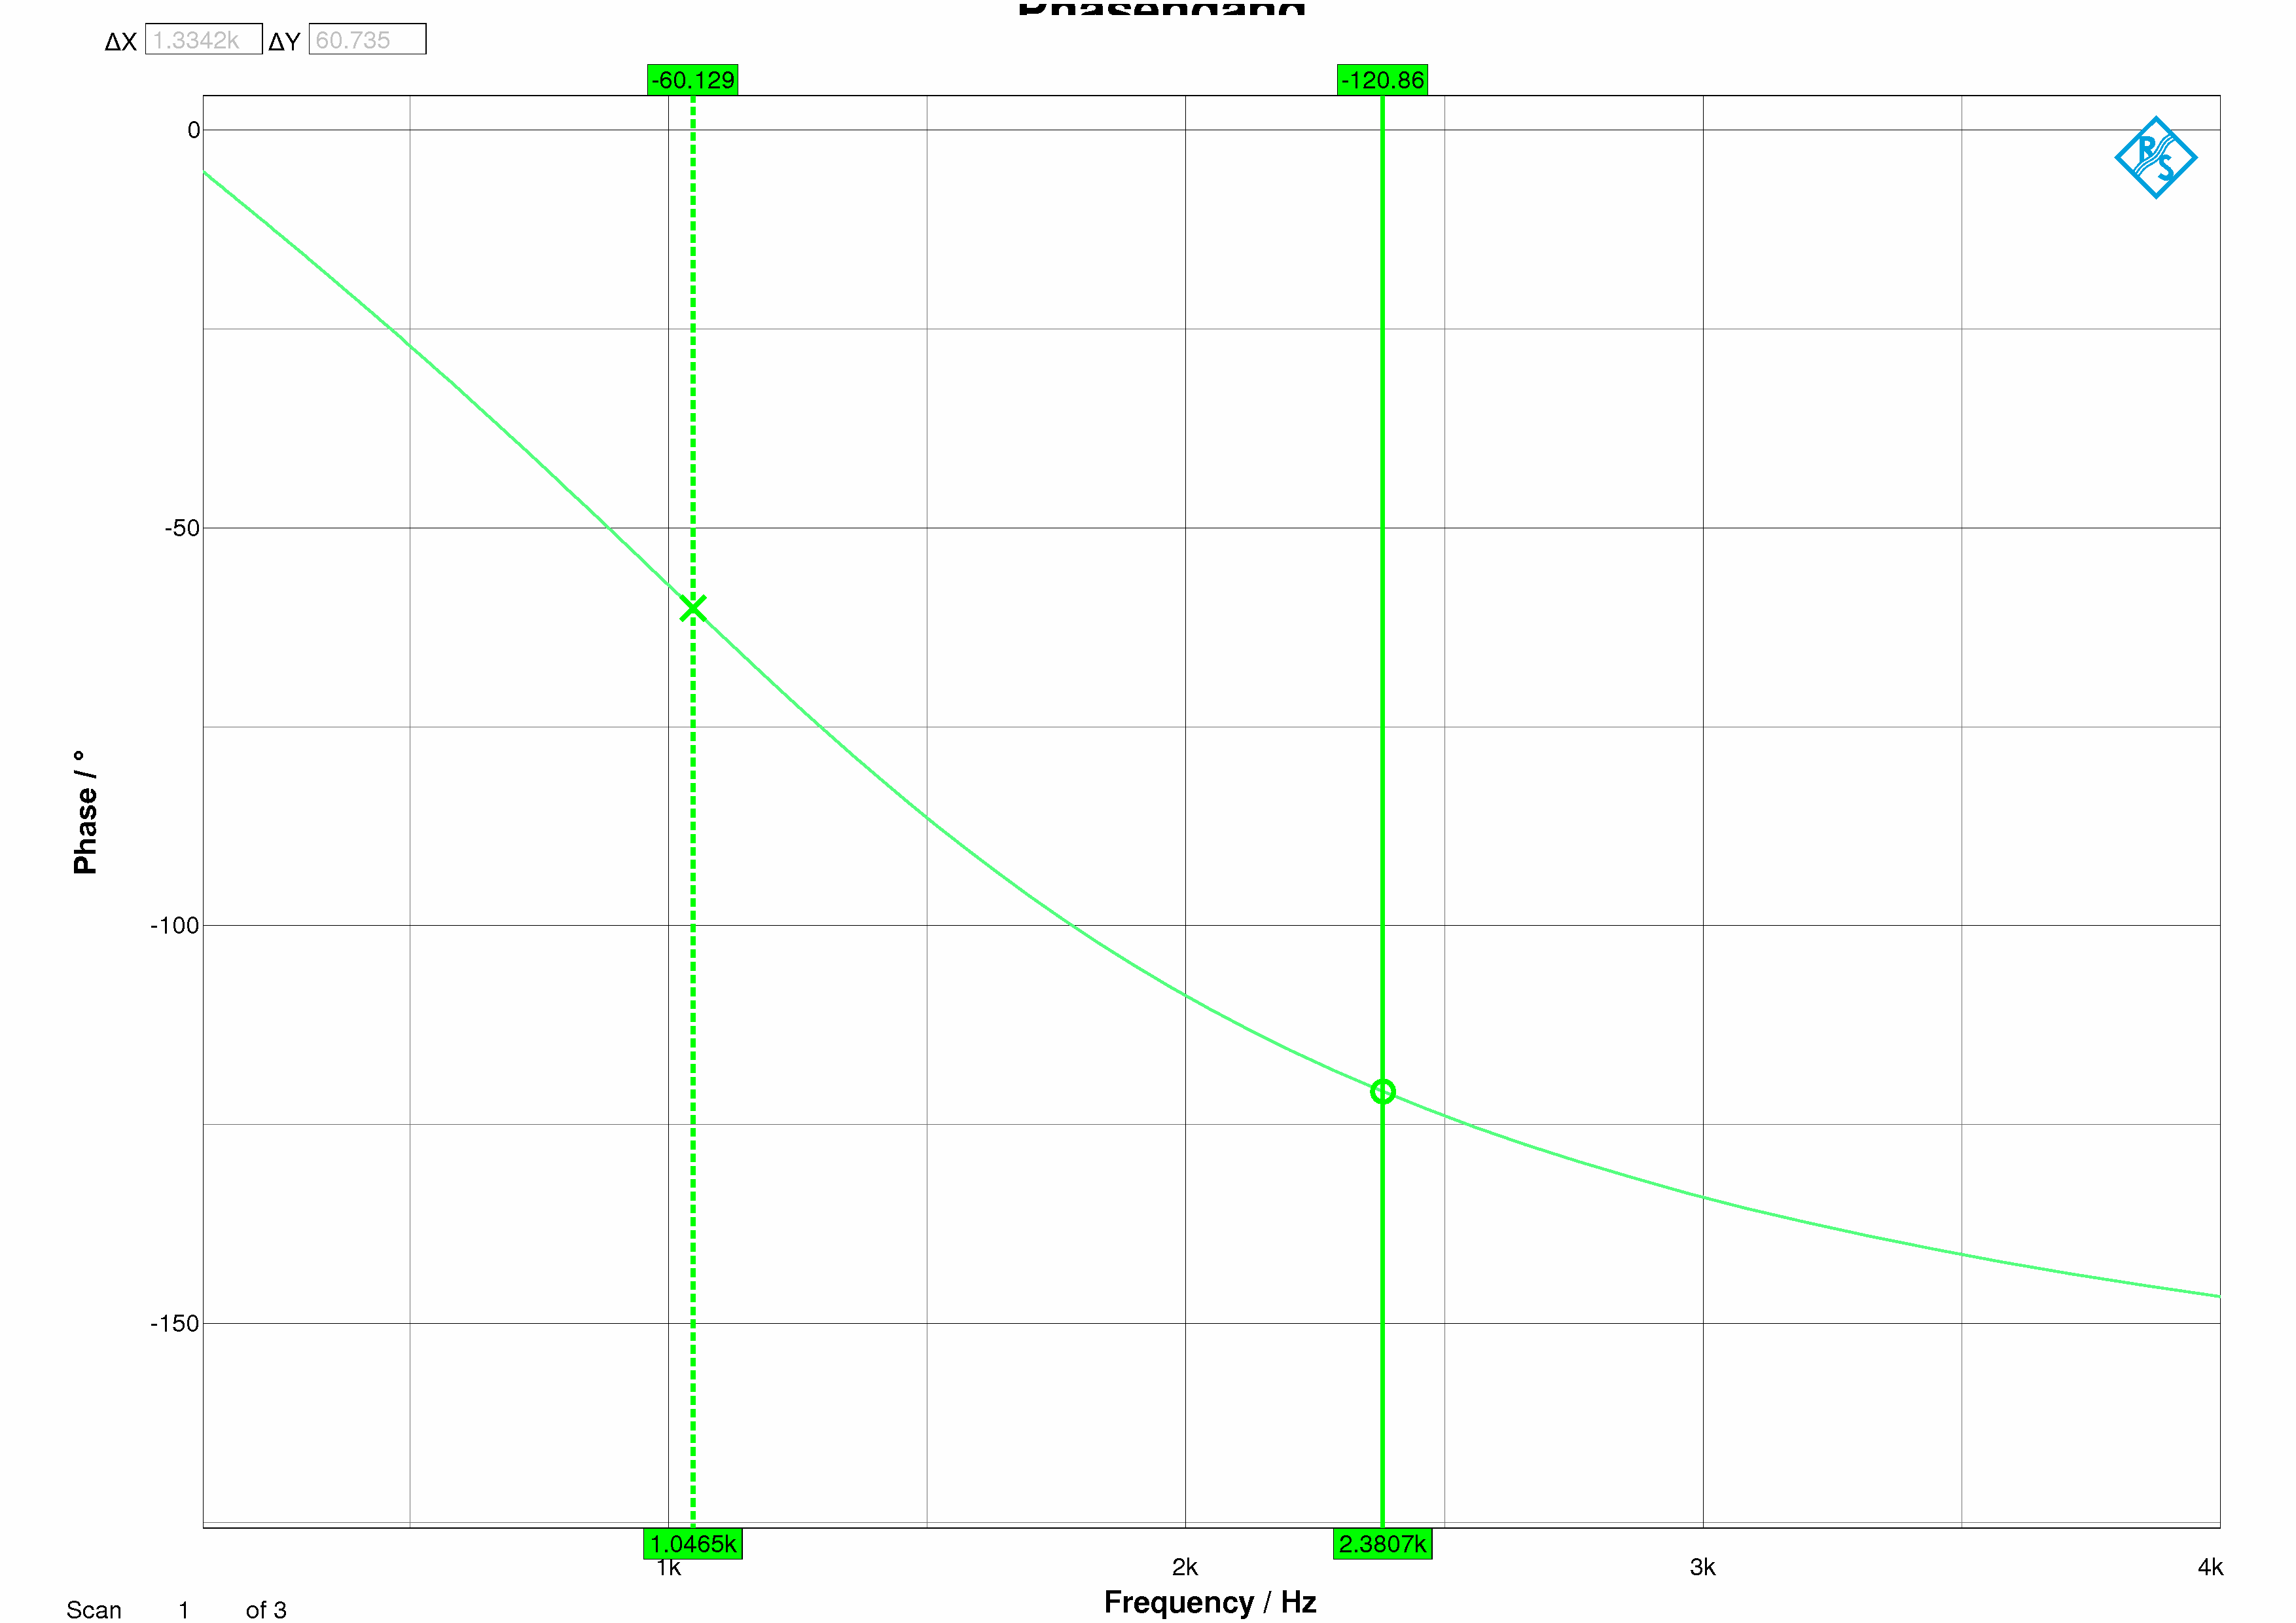
\includegraphics[width=0.65\linewidth]{Bilder/ImLabor/Phasengang_4_1_Butter_TP}
\caption{Phasengang Butterworth-Tiefpass mit Markern}
\label{fig:Phasengang_4_1_Butter_TP}
\end{figure}

\begin{figure}[h]
\centering
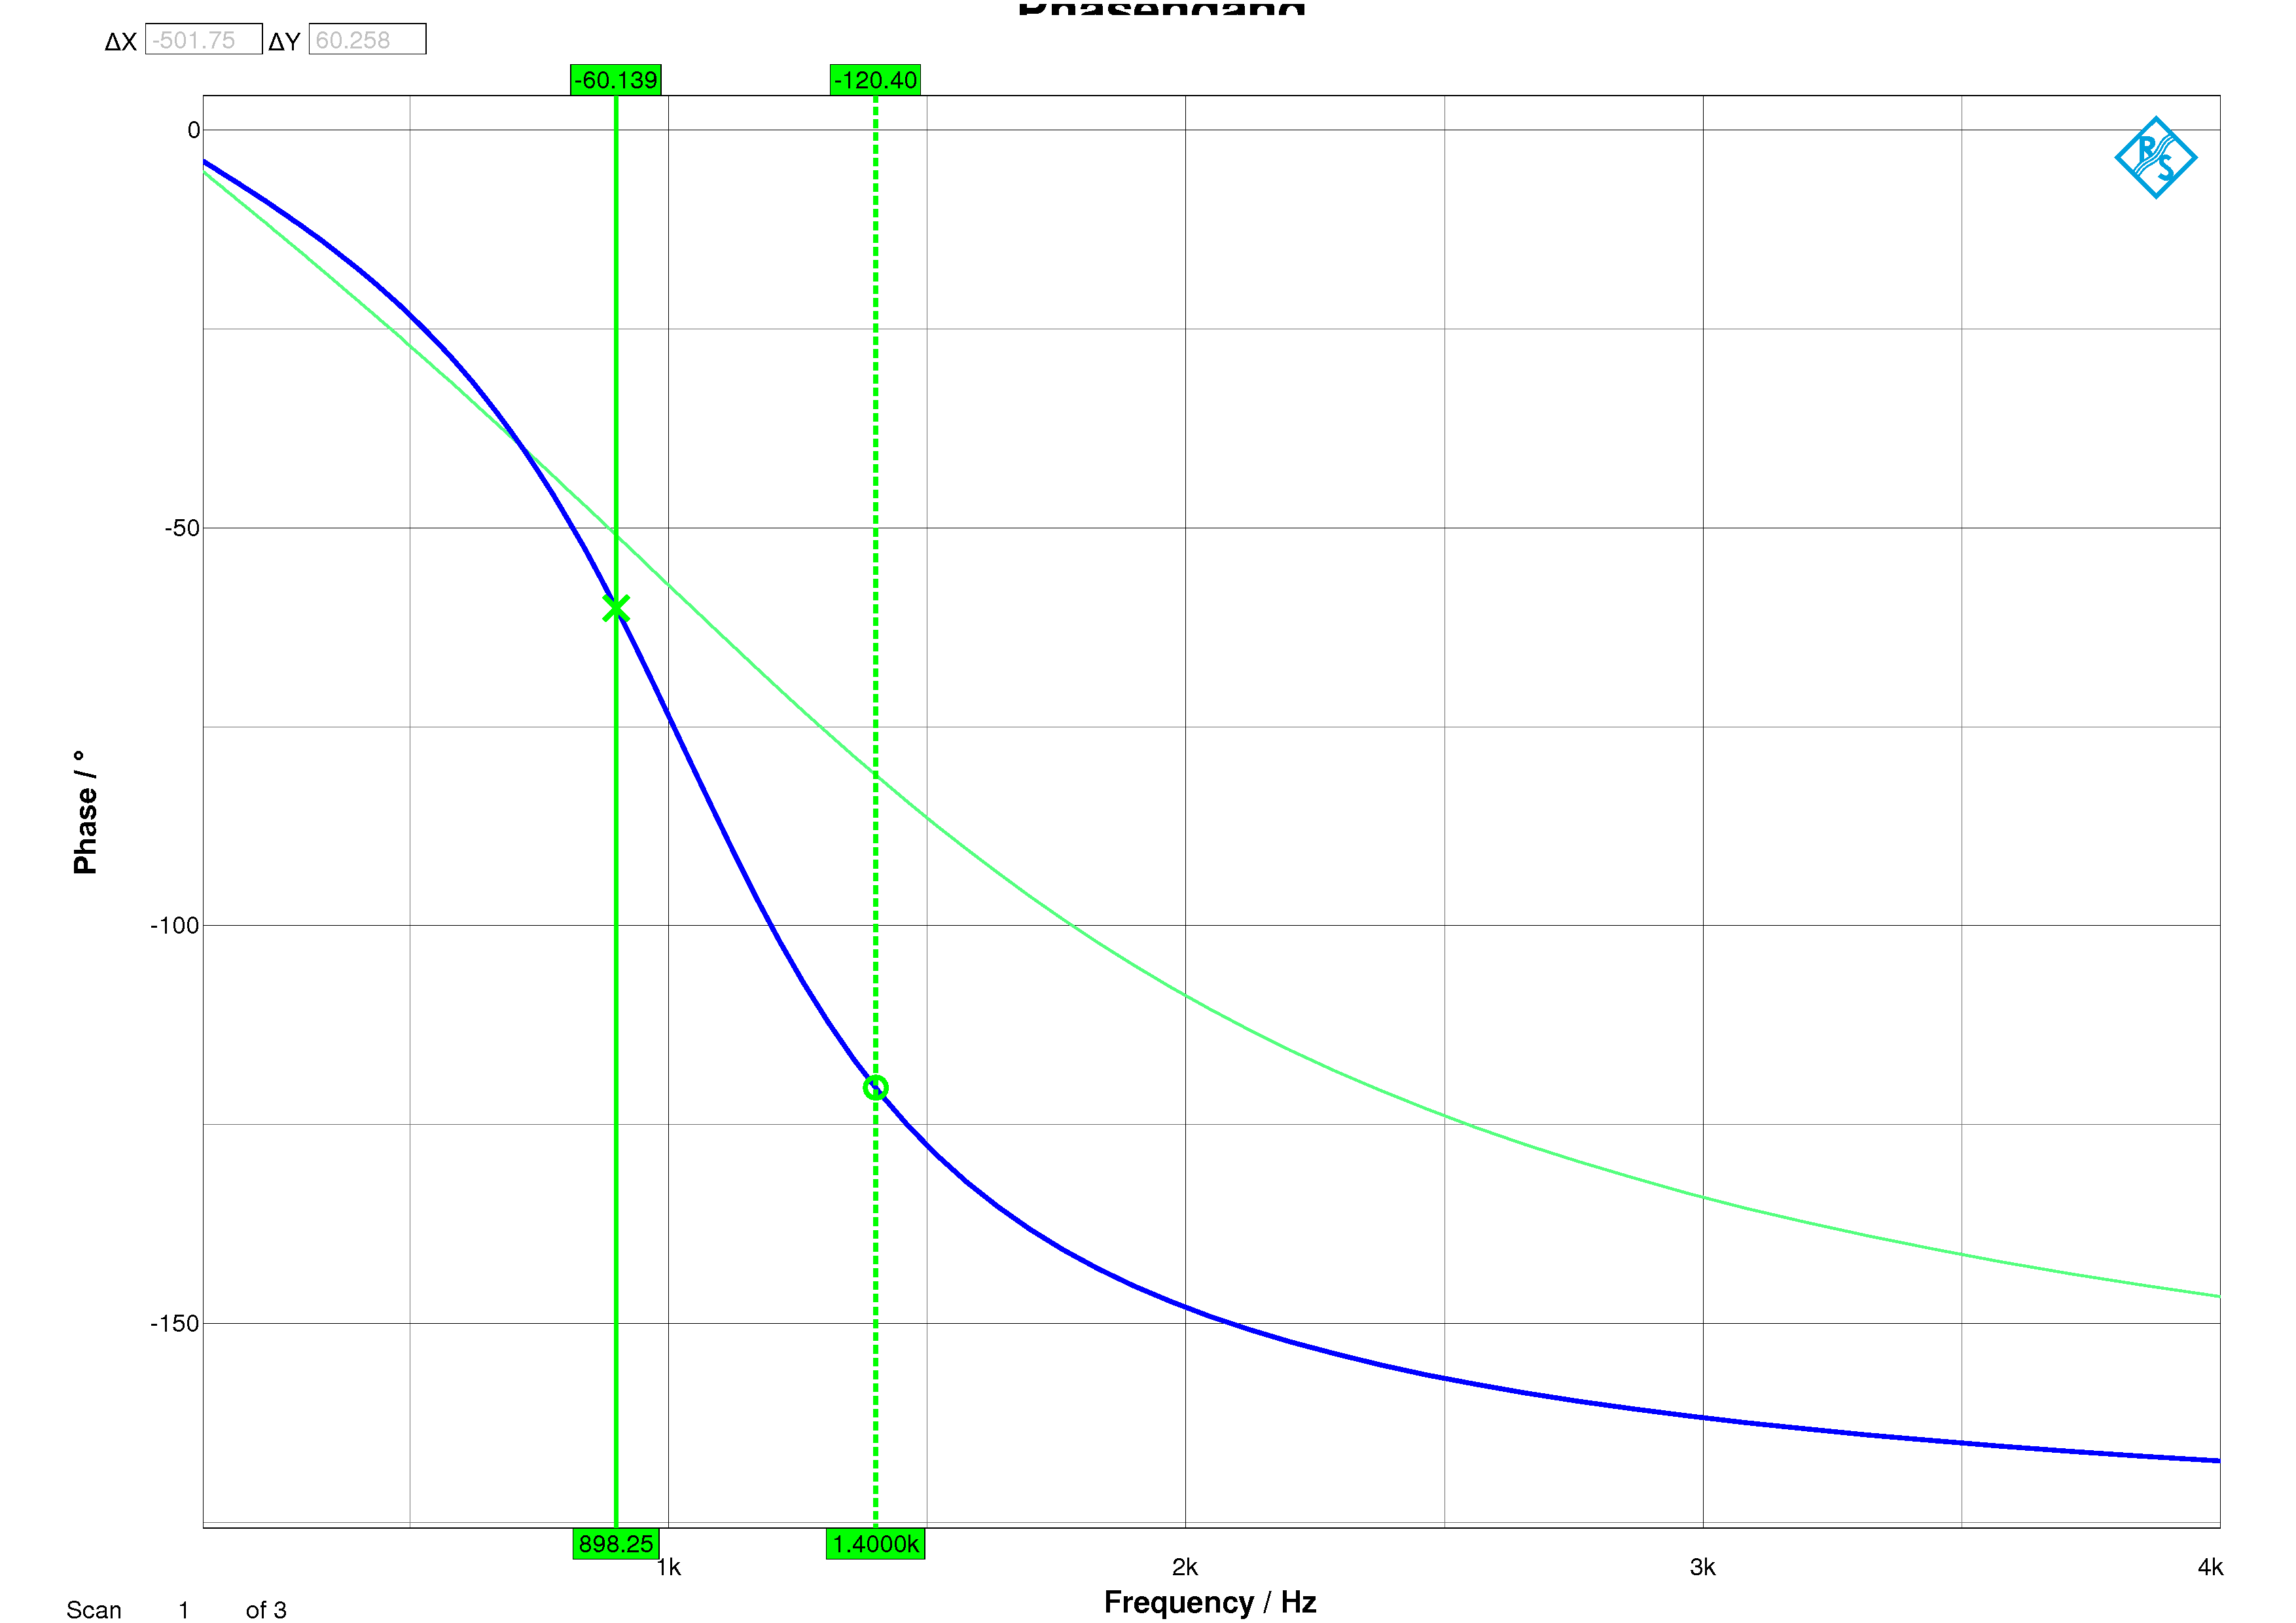
\includegraphics[width=0.65\linewidth]{Bilder/ImLabor/Phasengang_4_2_Tscheby_TP}
\caption{Phasengang Butterworth- und Tschebyscheff-Tiefpass mit Markern bei Tschebyscheff}
\label{fig:Phasengang_4_2_Tscheby_TP}
\end{figure}

\begin{figure}[h]
\centering
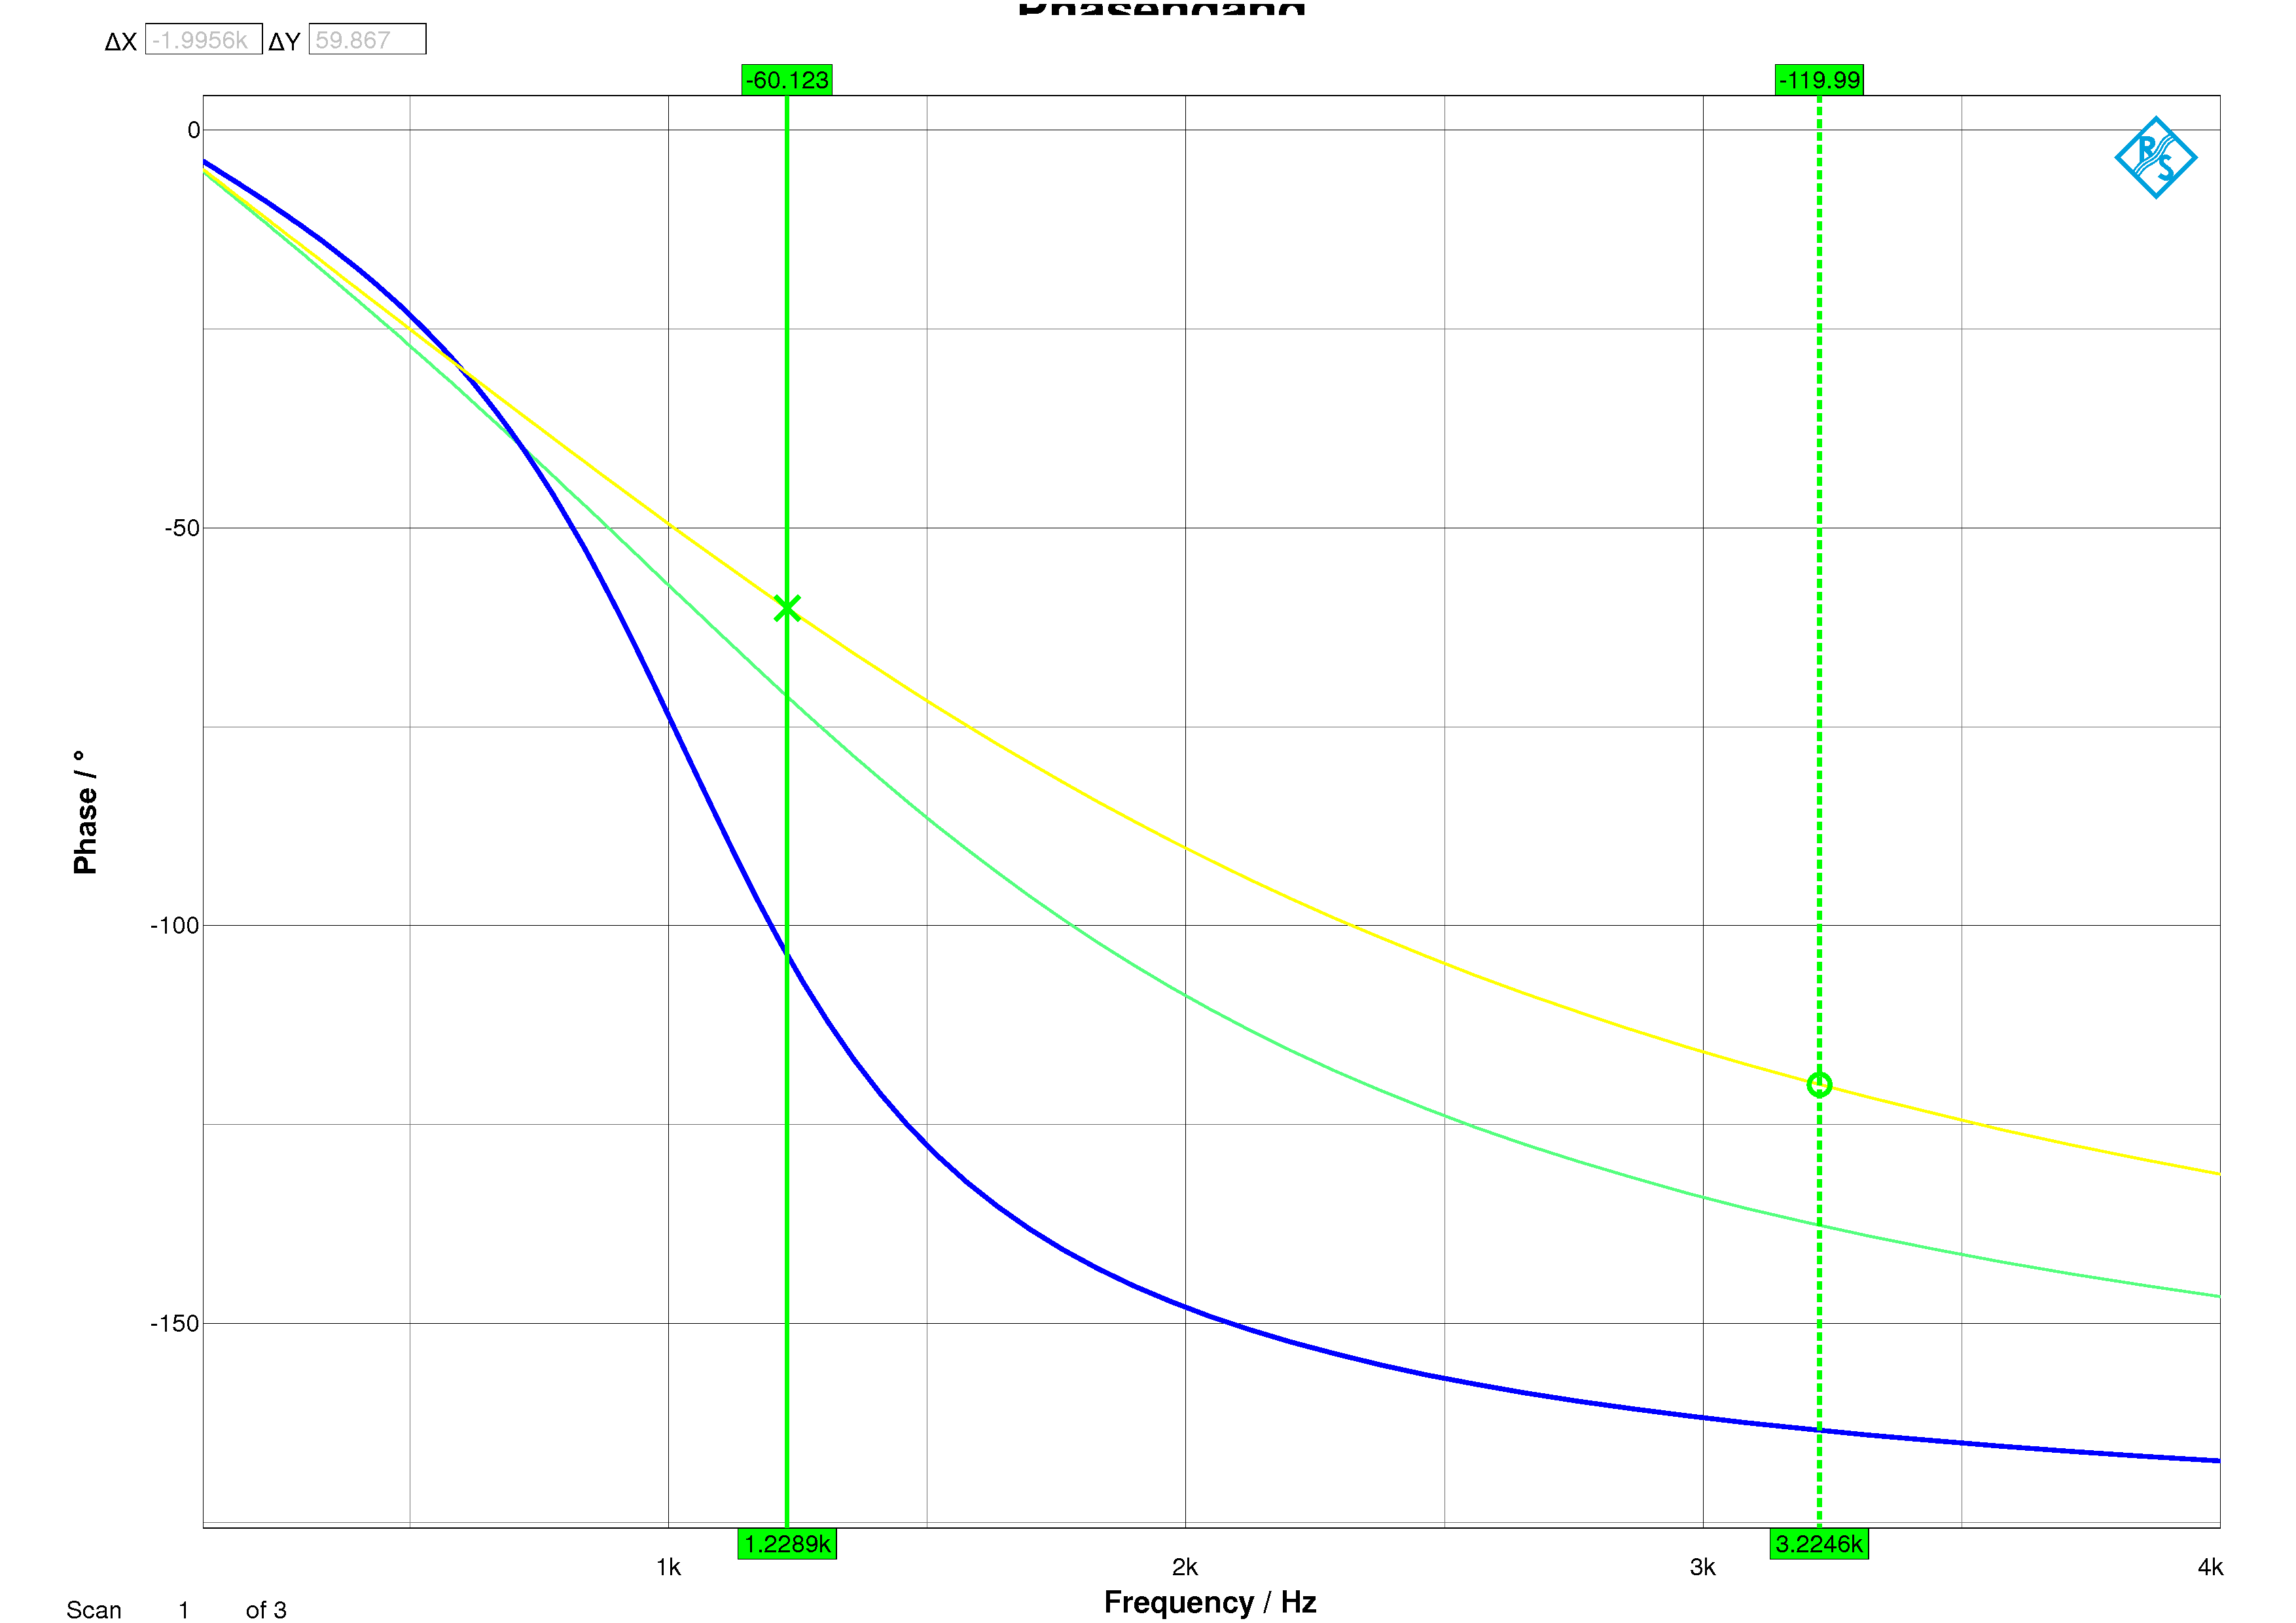
\includegraphics[width=0.65\linewidth]{Bilder/ImLabor/Phasengang_4_3_Bessel_TP_Alle}
\caption{Phasengang Butterworth-, Tschebyscheff- und Bessel-Tiefpass mit Markern bei Bessel}
\label{fig:Phasengang_4_3_Bessel_TP_Alle}
\end{figure}






\noindent \textbf{Unter folgenden Link kann eine \glqq Education\grqq~ Version von PSPice heruntergeladen werden.}
http://www.orcad.com/buy/orcad-educational-program


